\documentclass[11pt,a4paper,english]{scrreprt}
\usepackage[utf8]{inputenc}
\usepackage[T1]{fontenc}
\usepackage{lmodern}

\usepackage[english]{babel}
\usepackage{csquotes}
\usepackage[long,nodayofweek,level,24hr]{datetime} 
\usepackage[skip=5pt,font=footnotesize]{caption}

\usepackage{tabularx}
\usepackage{booktabs}
\usepackage{amsmath}
\usepackage{amssymb}
\usepackage{graphicx}
\usepackage{subfigure}
\usepackage{enumitem}
\usepackage{pdfpages}
\usepackage{xcolor}
\usepackage[bookmarksnumbered]{hyperref}
\hypersetup{pdfborder={0 0 0}, breaklinks=true}
\usepackage{bookmark}
% \addtokomafont{disposition}{\rmfamily}
\usepackage[onehalfspacing]{setspace}

% DISABLE TODO NOTES HERE %%%%%%%%%%%%%%%%%%%%%%%%%%%%%%%%%
\usepackage{todonotes}
%\usepackage[disable]{todonotes}

% HEADER & FOOTER DEFINITIONS %%%%%%%%%%%%%%%%%%%%%%%%%%%%%
\usepackage{fancyhdr}
\pagestyle{fancy}
\renewcommand{\headrulewidth}{0pt}
\fancyhead{}
\fancyfoot{}
\fancyfoot[R]{\textcolor{gray}{\thepage}}

\fancypagestyle{plain}{%
    \renewcommand{\headrulewidth}{0pt}%
    \fancyhf{}%
    \fancyfoot[R]{\textcolor{gray}{\thepage}}%
}

% LITERATURE %%%%%%%%%%%%%%%%%%%%%%%%%%%%%%%%%%%%%%%%%%%%%
\usepackage[backend=biber,style=apa]{biblatex}
\addbibresource{literatur.bib}


% DEF FOR COVER %%%%%%%%%%%%%%%%%%%%%%%%%%%%%%%%%%%%%%%%%%
\newcommand{\titelMAEnglish}{Explainable Artificial Intelligence:\\ Designing human-centric assessment system interfaces to increase explainability and trustworthiness of artificial intelligence in medical applications}

\newcommand{\authorMA}{Philipp Dominik Bzdok}

\newcommand{\examinerMA}{Univ.-Prof. Dr. rer. nat. Thomas Franke, Dipl.-Psych.}

\newcommand{\supporterMA}{Tim Schrills, M.Sc.}
%%%%%%%%%%%%%%%%%%%%%%%%%%%%%%%%%%%%%%%%%%%%%%%%%%%%%%%%%%%

% DEF FOR COMMENTS, CAN BE DELETED %%%%%%%%%%%%%%%%%%%%%%%%
\newenvironment{comment}
  {\par\medskip
   \begingroup\color{olive}%
   }
 {\endgroup
  \medskip}
%%%%%%%%%%%%%%%%%%%%%%%%%%%%%%%%%%%%%%%%%%%%%%%%%%%%%%%%%%

\begin{document}
\pagenumbering{gobble}
\begin{titlepage}
    \begin{figure}[t]
        \centering
        
\includegraphics[width=0.7\textwidth]{img/UzL_Logo.png}
    \end{figure}
    \todo{English Logo}
    \begin{center}
        \fontfamily{phv}\selectfont
        \textcolor{gray}{Director: Prof Dr. rer. nat. Michael Herczeg}\\
        \vspace*{1.5cm}
        \Large
        \begin{onehalfspace}
            \textbf{\titelMAEnglish}
        \end{onehalfspace}
        \vspace{1cm}
        \normalsize
        \textbf{Master's Thesis}\\
        \vspace{0.2cm}
        as part of the study program\\
        \textbf{Media Informatics}\\
        of the University of Lübeck\\
        \vspace{1cm}
        submitted by:\\ \textbf{\authorMA}\\
        \vspace{1cm}
        Issued and supervised by:\\ \textbf{\examinerMA}\\
        \vspace{0.5cm}
        with support from:\\ \textbf{\supporterMA}\\
        \vspace{1cm}
        Lübeck, \today
    \end{center}        
\end{titlepage}
\setlength{\parindent}{0em}
\setlength{\parskip}{1em}

\begin{comment}
\begin{center}
    \textbf{Vorbemerkung}

    (Version: 2021-05-12-IMIS LaTex Version by Philipp Bzdok)
\end{center}
Anbei ein kommentiertes Template für Projekt- und Abschlussarbeiten in der Medieninformatik. Die grünen Kommentare in jedem Fall vor einer (Zwischen-) Abgabe entfernen (alle!).

Alle Angaben sind eigene Einschätzung (bzw. aus den zitierten Quellen, die aber auch wieder nach eigenen Überlegungen von mir ausgewählt wurden) und entsprechend ohne Gewähr. Nordstrom's Policy gilt auch hier: "Use your own best judgment at all times.".

Es ist ihre Arbeit. Sie investieren 6 Monate Ihrer Lebenszeit in die Arbeit und Sie müssen Sie vor anderen verteidigen. Sehen Sie Hinweise von anderen als Ratschläge: Ernst nehmen, aber immer für sich selbst entscheiden, was passt, was nicht und was auf ein Problem hinweist, was man dann aber anders löst.
Das letzte Wort (v.a. über formelle Aspekte) hat allerdings immer der jeweilige Betreuer.

Zunächst kommen ein paar allgemeine Vorbemerkungen, die für die ganze Arbeit relevant sind (Allgemeine Punkte der Arbeit). Danach die Gliederung einer normalen Arbeit mit Anmerkungen in den entsprechenden Kapiteln bzw. Abschnitten.

Viel Erfolg beim Schreiben.

Daniel Wessel

\textbf{Rundumschlag was wissenschaftliches Arbeiten betrifft:}\\ \url{https://www.youtube.com/watch?v=_ID7q7pXzyc}

\textbf{Allgemeine Punkte der Arbeit}
\begin{itemize}
    \item \textbf{Änderbarkeit von Struktur und Inhalten:} Je nach konkretem Thema kann eine andere Struktur sinnvoll sein. Dies ist ins-besondere bei der Reihenfolge der Analyse-Abschnitte der Fall, kann aber auch ganze Kapitel betreffen. Das ist insbesondere bei Masterarbeiten der Fall, die sich je nach Ausrichtung (z. B. theoretische Arbeit) stark von der sonst üblichen Form unterscheiden. Diese Struktur so früh wie möglich mit dem Betreuer klären, ihm dann per eMail zuschicken und sich kurz bestätigen lassen (generell hat man viel zu tun und erinnert sich nicht unbedingt an alle Absprachen, deswegen einfach im Anschluss kurz eine Zusammenfassung des Gesprächs per eMail schicken).
    \item \textbf{Exposé (Bachelor-/Masterarbeit) bzw. Pflichtenheft (Bachelor-/Masterprojekt) setzt die inhaltliche Bewertungsgrundlage:}  Darin haben Sie (Arbeit) oder Ihr Betreuer (Projekt) festgelegt, was zu erreichen ist. Entsprechend genau überlegen, was man verspricht bzw. zu was man sich verpflichtet.
    \item \textbf{Zielgruppe:} Schreiben Sie die Arbeit so, dass andere Personen verstehen, was Sie machen — auch wenn sie keine (Medien-)Informatik studiert haben. Sprich: Beginnen Sie breit um den Einstieg zu erleichtern und formulieren Sie es allgemein verständlich (z. B. das die öffentliche Verwaltung zunehmend digitalisiert wird) und fassen Sie am Ende eines Kapitels die Punkte allgemeinverständlich wieder zusammen. Dazwischen können Sie auf ein Detaillevel runtergehen und eine Komplexität nutzen, die ein Laie nicht mehr versteht. Da der Text in Absätzen aufgebaut ist, kann der Laie (oder nicht interessierte) diese Absätze überspringen. Der Laie sollte aber zumindest im Prinzip verstehen, was Sie gemacht haben.
    \item \textbf{Roter Faden:} Die Arbeit logisch aufeinander aufbauen: In der Einleitung legen Sie dar, was Sie erreichen wollen und zeigen dabei auch subtil, warum das wichtig / interessant / relevant ist (\textit{"Why should I care?"}). Das geschieht über Belege und Argumente, wann immer Sie "wichtig", "interessant" oder "relevant" im Text verwenden sind Sie dabei gescheitert. \textbf{Alle} Kapitel nach der Einleitung zeigen \textbf{logisch aufeinander folgend}, wie der Zweck der Arbeit erreicht wird.
    \item \textbf{Zwischenstufen-Denken:} So schreiben, dass am Ende jedes Kapitels (Einleitung, Analyse, Konzeption, Realisierung, Dialogbeispiele, Evaluation) der Leser stoppen könnte und die Arbeit selbst fortführen könnte (z. B. nach der Einleitung sich für eine anderes Analysevorgehen entscheiden, oder auf Basis der Analyse eine andere Lösung konzipieren).
    \item \textbf{Eigenes Fazit am Ende jeden Kapitels — Was bedeuten die Ergebnisse für die Arbeit bzw. deren Ziel?} Z. B. am Ende der Analyse kurz zusammenfassen, was die wesentlichen Punkte für die weitere Entwicklung sind — mit Fokus auf das nächste Kapitel (hier: Konzeption). Am Ende der Konzeption kurz zusammenfassen, was die wesentlichen Punkte für die weitere Entwicklung (jetzt: Realisierung) sind, etc. pp. Ein gutes Fazit ist viel Arbeit und setzt ein gut geschriebenes Kapitel voraus.
    \item \textbf{Professionelle Zwischenabgaben:} Wenn Sie den Text an den Betreuer geben, gehen Sie vorher kritisch drüber. Wenn Textmarken falsch gesetzt sind, die Formatierung zusammengebrochen ist, etc. dann muss sich der Betreuer da erst mal durchwühlen um zum Inhalt zu kommen. Gute Formatierung macht keine schlechte Arbeit gut (die inhaltlichen Fehler fallen eher umso deutlicher auf), aber schlechte Formatierung macht eine gute Arbeit schlechter.
    \item \textbf{Professionell und offen Kommunizieren:} Weder sich selbst kreuzigen noch Fehler verbergen, sondern berichten, was gemacht wurde und mit Fehlern konstruktiv umgehen.
\end{itemize}

\textbf{Sprache: Stil}
\begin{itemize}
    \item \textbf{Kein Ich, keine Hero's Journey:} Es ist — im Prinzip — egal, wer die Arbeit durchgeführt hat (zumindest für die Qualität der Arbeit, nicht für die Bewertung Ihrer Leistung). Was überzeugen muss ist das Vorgehen, die Belege und Argumentation. Entsprechend stellen Sie das Vorgehen neutral dar ohne auf sich selbst zu verweisen (eher passiv verwenden). Ausnahmen sind u.a. in Danksagung, Widmung, Eidesstattliche Erklärung.
    \item \textbf{Meta vermeiden}: Sie müssen an vielen Stellen darauf hinweisen was kommt (z. B. zu Beginn eines jeden Kapitels). Reißen Sie den Leser aber dabei nicht aus dem Text. Mental ist der Leser dabei, ihre Arbeit zu beobachten, was Sie konkret getan haben. Wenn Sie ihm jetzt sagen "In diesem Kapitel ..." dann ziehen Sie ihn aus dem Text und bringen ihn dazu, über den Text nachzudenken statt über das, was gemacht wurde. Bleiben Sie bei dem, was Sie gemacht haben, z. B. "Nachfolgend werden ...". 
    \item \textbf{Kapitel $\neq$ Unterkapitel $\neq$ Abschnitt:} 1 ist ein Kapitel, 1.1 ein Unterkapitel, 1.1.1 ein Abschnitt, 1.1.1.1 existiert nicht. Wenn Sie noch mehr Einteilungen brauchen, dann verwenden Sie Abschnitte mit Fettdruck zu Beginn (wie in diesem Abschnitt, dann aber ohne die Bulletpoints).
    \item \textbf{Kein Bulletpoint-Text:} Bulletpoints sind nur an wenigen Stellen hilfreich, z. B. bei Aufzählungen. Sätze nie mit Bulletpoints aufzählen. Entweder die Sätze auf Stichworte reduzieren oder eine Tabelle draus machen.
    \item \textbf{Auch digital gedrucktes ist tot und macht nichts mehr:} Sie berichten was Sie gemacht haben — außerhalb des Berichtes. Entsprechend nie schreiben, dass z. B. in der Analyse der Sachverhalt analysiert wird. Der Bericht macht von sich aus nichts. Sie stellen dort die Ergebnisse der Analyse dar.

    \item \textbf{Umgangssprache vermeiden, Hochgestochene Sprache vermeiden:} Weder Umgangssprache (Sozialpädagogensprache; "tut", "Das Ganze ...", "etwas für ihre Gesundheit zu machen") noch Hochgestochen (à la Philosophendeutsch) schreiben. Wissenschaftliche Sprache ist nach \textcite{alley_1996}:
    \begin{itemize}
        \item präzise: sagen was man meint (richtige Wort, richtiges Detaillevel)
        \item klar: vermeiden Sachen zu sagen/implizieren, die man nicht meint, d.h. Ambiguität und unnötige Komplexität (v.a. in der Wahl der Wörter) vermeiden
        \item ehrlich: direkt und offen kommunizieren
        \item prägnant: jedes Wort sollte zählen
        \item bekannt/vertraut: neue Fakten in bekannten Kontext verankern
        \item flüssig: von Satz zu Satz, Absatz zu Absatz, ohne dass der Leser stolpert
    \end{itemize}
    \fullcite{alley_1996}
\end{itemize}

\textbf{Sprache: Zeitformen}
\begin{itemize}
    \item \textbf{In einem Bericht berichten Sie:} Entsprechend Vergangenheitsform verwenden. Sie berichten über eine abgeschlossene Arbeit, selbst wenn diese noch läuft als Sie es geschrieben haben, und selbst bei Zielen der Arbeit. Ausnahmen sind selten, z. B. bei den Ergebnissen ("Daten zeigen ..." — sie machen es ja noch) und Aus-blick bzw. Vorschläge für die Zukunft.
\end{itemize}

\textbf{Sprache: Absätze}
\begin{itemize}
    \item \textbf{Eine Sinneinheit = 1 Absatz:} Absätze behandeln immer einen Punkt, eine Sinneinheit. Wenn eine halbe Seite lang kein Absatz verwendet wird, liegt meist ein Problem vor.
    \item \textbf{Absätze sind immer länger als ein Satz:} Keine Einsatz-Stückel-Absätze. Einzige Ausnahme: Sie wollen, dass der Leser die komplette Aufmerksamkeit auf diesen zentralen Satz lenkt. Das kann man 1-2 Mal in einer Arbeit machen.
\end{itemize}

\textbf{Interne Verweise}
\begin{itemize}
    \item \textbf{Verweise statt Wiederholungen:} Üblicherweise braucht man einen Sachverhalt nur ein Mal zu beschrieben — dann verweist man an anderer Stelle auf den konkreten Abschnitt. Das ist auch der Grund für die Nummerierung — es erlaubt Ihnen, den Leser präzise zu den Punkt in der Arbeit zu schicken, an dem Sie auf den Sachverhalt eingehen. Nutzen Sie also "wie in der Kontextanalyse (2.4) beschrieben ...", dann weiß der Leser, wie lange er blättern muss.
\end{itemize}

\textbf{Zitationen}
\begin{itemize}
    \item \textbf{APA verwenden:} American Psychological Association (7. Ausgabe) Stil verwenden. Gibt genug Informationsseiten dazu im Netz und Literaturmanager können diesen Stil üblicherweise.
    \item \textbf{Richtige Zitationen:} Falsche "ich füg die richtigen Zitationen später ein" Ab-gaben verbrennen Ihnen den Betreuer. Arbeiten Sie von Anfang an mit einem Literaturverwaltungsprogramm, in dem die verwendeten Quellen richtig eingetragen sind (nächster Punkt).
    \item \textbf{Autorennamen müssen genannt werden, aber nicht hervorheben:} Die Wissenschaft sollte keinen Personenkult kennen — das können gerne Religionen oder Ideologien übernehmen. Wer was herausgefunden hat, ist egal. Die Qualität der Arbeit zählt. Entsprechend nicht "Die Autoren xyz haben herausgefunden das ABC vor-liegt" sondern "Da ABC vorliegt (Autoren Jahr) ...".
    \item \textbf{Kein Paper-Denglish:} Ja, im englischen heißt es Paper. Im Text sind es aber Artikel oder Konferenzbeiträge oder Buchkapitel oder was auch immer. Üblicherweise muss man den Typ auch nicht erwähnen (im Normalfall wurde man eh Artikel/Konferenzbeiträge zitieren). Bitte nicht so was wie "Im Paper von xyz ...", das klingt nach Möchtegern-coole Manta mit Fuchsschwanz Sprechweise. Ein-fach berichten wie die Befundlage ist, über Autorenname und Jahr (meist in Klammern) belegen wo es herkommt (sonst ein Plagiat) und die Belege und Argument in der Arbeit sprechen lassen.
    \item \textbf{Wörtliche Zitate nur wenn es nicht anders geht:} In den meisten Fällen geben Sie Befunde oder Argumente mit Ihren eigenen wieder (mit Quellenangabe). Wörtliche Zitate braucht man nur in sehr seltenen Fällen. Z. B. treffende Aussage von Evaluationsteilnehmern, oder eine Definition, die man 1:1 so sagen muss.
    \item \textbf{Fußnoten vermeiden:} Entweder es ist wichtig genug, genannt zu werden, oder es ist so unwichtig, dass es raus kann. Fußnoten reißen den Leser aus dem Text. Einzige Ausnahme: Bei der ersten Verwendung des generische Maskulinums.
    \item \textbf{Es gibt mehr Plagiate als nur Quellen nicht angeben:} Es gibt z. B. Übersetzungsplagiate, bei denen Sie einen Text(teil) einfach auf deutsch übersetzen ohne die Quelle anzugeben, oder dass man einfach die Argumentstruktur und Quellenangaben aus einem anderen Text übernimmt (ohne die Quelle anzugeben). Sie schmücken sich dann mit fremden Federn und Blender sind selten willkommen.
    \item \textbf{Literaturverwaltungsprogram nutzen:} Literaturverwaltungsprogramm (z. B. Zotero) hilft extrem bei der richtigen Zitierung, aber ACHTUNG: Wenn die Angabe in Zotero fehlt, ist auch die automatische Generierung des APA Stils falsch! GIGO gilt auch hier.
\end{itemize}

\textbf{Abbildungen und Tabellen}
\begin{itemize}
    \item Expliziter Verweis vom Text auf die Abbildung/Tabelle immer im Absatz vor der Abbildung/Tabelle (Leser stolpern über Abbildung/Tabelle, suchen dann nach oben nach mehr Informationen).
    \item Auf \textbf{Lesbarkeit} achten! Schriftgröße und Auflösung (bei Bildern) im Probedruck überprüfen!
    \item Für Schwarz/Weiß-Druck und für Farbfehlsichtige geeignet.
    \item Tabellen nach \textbf{APA Stil} (nur horizontale Linien und nur nach Header oder vor Footer.
\end{itemize}

\textbf{Druck}
\begin{itemize}
    \item Arbeit einseitig drucken!
    \item \textbf{PDF Druck und Suchfunktion:} Zuerst als PDF drucken, dann nach "Fehler! Verweisquelle konnte nicht gefunden werden." suchen. Word bricht schon mal gerne die Verlinkungen und das sieht man erst im Druck! Generell PDF Dokument kritisch durchgehen und PDF auch zum Drucken im Copyshop verwenden!
    \item Nach dem Druck und vor dem Binden alle Seiten selbst sowie von einer anderen Person durchgehen (lassen).
\end{itemize}
\end{comment}
\newpage
\chapter*{Danksagung}
\begin{comment}
Kurzer Dank an Personen, die Sie bei der Arbeit unterstützt haben. Z. B. inoffizielle Betreuer, Teilnehmer an den Evaluationen (nie namentlich nennen), Medientechnik, Sekretärin, etc. pp. — nur wenn Sie den Personen wirklich dankbar sind. (Ist nett aber für die Bewertung irrelevant.)
Falls nicht verwendet diese Seite einfach entfernen.
\end{comment}

Text \dots

\newpage
\chapter*{Kurzfassung}
\begin{comment}
Abstract schon für Zwischenabgabe schreiben. Später kommen dann noch Sätze dazu, aber Grundgerüst steht.

Kein "Teaser" sondern eine kurze Zusammenfassung (das, was man braucht, um sich schnell einen Überblick zu verschaffen, ob es sich lohnt, die Arbeit zu lesen).

Inhalt umfasst die zentralen Punkte aller Kapitel, von Ziel/Fragestellung bis Ausblick.

Nie länger als diese eine Seite (inkl. Schlüsselwörter).
\end{comment}

Text \dots

\section*{Schlüsselwörter}
\begin{comment}
Verwendete Literatur gibt Hinweise auf passende Stichwörter. Das sind die Suchbegriffe, die man bei einer Literatursuche verwenden würde.
\end{comment}

Text \dots

\newpage
\chapter*{Abstract}
\begin{comment}
Englische Version der Kurzfassung.
Nicht einfach Google Translate oder DeepL verwenden. Trifft die Nuancen nicht und klingt z. T. nach Yoda.
\end{comment}

Text \dots

\section*{Keywords}
Text \dots

\newpage
\tableofcontents

\newpage
\pagenumbering{arabic}
\chapter{Introduction}\label{chapter:introduction}
The use of modern Artificial Intelligence (\textbf{AI}) techniques is pervasive and can be found in many fields of application, such as digital image processing, search engines and speech recognition \parencite{eu_com_ai}. Other application fields, such as medical diagnosis systems, cannot benefit as easily from AI-based technology compared to recreational domains. This impediment stems oftentimes from the AI being a "black box". In consequence humans struggle to understand such AI-systems and their output, leading to trust and compliance issues \parencite{adadi_blackbox_2018}. These issues are further enhanced in the medical context where decisions, possibly based on AI, can have severe consequences for users, especially patients.

An example for medical human-AI-interaction is the image-based recognition of Deep Vein Thrombosis (\textbf{DVT}) with real time AI support for medical professionals by \textit{Think\-Sono}. The system leverages AI to guide the user through the current gold-standard diagnosis, a compression ultrasound examination, so that it enables any healthcare professional to detect DVT \parencite{thinksono_website}. Closely related in this context is the interdisciplinary research project \textit{CoCoAI}, which aims to explore psychological, ethical and technological implications of human-centered, AI-based applications in the DVT diagnosis and beyond \parencite{cocoai_website}. 

When AI-based systems are used in high risk application contexts, such as medical diagnosis, the aspects of explainability, interpretability and trustworthiness become a primary concern for adoption and use of said system. \textcite{ribeiro_why_2016} already explored the importance of explainability and trust in AI-based systems and postulated that AI systems will not be used if the users have no trust in the model or the results. Even though many machine learning algorithms score high on standard performance metrics, such as precistion, recall or Area Under the Receiver Operating Characteristics (\textbf{AUROC}), user-facing performance may be way worse \parencite{gordon_disagreement_2021}. Understanding the AI's underlying machine learning (\textbf{ML}) model and its predictions is an important step for assessing trust and facilitating effective interaction \parencite{ribeiro_why_2016}. Recent technological advances are realized by \textit{Clearbox AI}, with the focus on trustworthy AI by implementing an AI model assessment \parencite{clearbox_website, eu_trustworthy_ai}. The model assessment can help model owners to identify robustness issues, potential undesired behaviour, and explain errors and uncertainties regarding the model predictions \parencite{clearbox_wp}.

Trust in AI systems is primarily induced by the users' understanding and the general interpretability of the machine learning model and their predictions \parencite{ribeiro_why_2016, ras_explanation_2018}. The wide array of different possible user groups and the complex constructs of understandability and trust demands for a human-centric approach in designing AI assessment systems. Because of the inherent complexity of non-linear machine learning models, especially Deep Neural Networks (\textbf{DNNs}) for image processing, suitable visualization and communication techniques are non-trivial. Additionally to the complex models for image classification, the input data is also more complex as it is unstructured. Non-linear neural networks and unstructured data provide additional challenges for Explainable Artificial Intelligence (\textbf{XAI}), as described in \textcite{keane_how_2019}. XAI is a research field that studies how AI decisions and data driving those decisions can be explained to people in order to provide transparency, enable assessment of accountability, demonstrate fairness, or facilitate understanding \parencite{arrieta_explainable_2019}. XAI plays an important role in the acceptance and finally in the usage of AI-based technology. This is further underlined in the medical context where public authorities set strict regulations on the usage of technological systems and ethic concerns have to be thoughtfully addressed.

In the context of a image-based medical diagnosis system, it is important that the responsible stakeholders, such as medical practitioners, specialized doctors and clinic managements, are enabled to make informed decisions on the usage of AI-based technology, even though their expertise in machine learning and data science is expected to be low. The stakeholders' trust in this system is a primary factor for the widespread use of said technology for real life applications. Therefore, increasing the understanding of the AI model and finding an optimal trust level in the predictions by designing human-centric explanation techniques within the AI model assessment system is a main goal of this work. Additionally it is conceivable that authorities will instantiate auditors for AI-based systems in medical contexts. Having a comprehensible and scientifically proven assessment system could be a big step in the approval and adoption of said system. 

\section{Goals}
The users understanding of the AI model and trust in the model are highly essential as pointed out by \textcite{knapic_explainable_2021}. This holds especially true for medical applications where re-traceable results have to be provided and people acting on these results bear great responsibility. To facilitate understanding and trust the machine learning model has to be interpretable and explainable. In the context of Convolutional Neural Networks (\textbf{CNNs}) interpretability of models can pose a significant concern because of their inherent complexity. Explanations of AI-models can provide insights on the machine's decision process and therefore generate user understanding. This can lead to the model being more interpretable by humans.

Assessing the suitability and performance of a CNN for a specific task by applying standard performance evaluation metrics is problematic, since these can be oblivious to distinguishing the diverse problem solving behaviors of a neural network \parencite{lapuschkin_unmasking_2019}. \textcite{samek_explaining_2021,JMLR:v17:15-618,ribeiro_anchors_2018} give an overview on the technical foundations of XAI and a presentation of practical methods, which will be used in conjunction with human-centric design to explore and evaluate suitable and efficient methods to explain a model's classification.

The goal of this thesis is to design, develop and evaluate interactive AI-assessment-system artifacts for medical professionals and machine learning specialists in a human-centric fashion to facilitate understandability and trustworthiness of AI-models. Developing such a system, with human concerns in focus, leads to following research questions:
\begin{itemize}
    \item[Q1:] How is the stakeholders' (medical professionals, clinic managements or data scientists) subjective information processing awareness linked to trust for a specific model and its predictions in the medical domain?
    \item[Q2:] How can different explanation techniques, ranging from perturbation based approaches to more model intrusive alternatives, increase trust in image classifier models and predictions?
    \item[Q3:] What are the most efficient methods to explain and possibly optimize trust levels in image classification models?
    \item[Q4:] To what extend can structured metadata increase the stakeholder's understanding of a model's operational range and performance?
\end{itemize}

\section{State of the Art}\label{section:state_of_the_art}
An AI-assessment-system is currently offered by Clearbox AI. The \textit{AI Control Room} cloud platform enables users to assess, improve and validate ML models and data in accordance with the principles of Trustworthy AI \parencite{clearbox_website,eu_trustworthy_ai}. \textcite{clearbox_website} describes its AI-assessment-system as a "Deep Pre‑production Analysis" tool:
\begin{displayquote}
    "AI Control Room automatically generates a model assessment to help model owners to identify robustness issues, potential undesired behaviour, and explain errors and uncertainties regarding the model predictions."
\end{displayquote}

Concretely the product enables users to perform following tasks for AI models working on tabular data:
\begin{description}
    \item [Model behaviour validation:] Validation metrics and plausible causes of error are clearly presented, potential limitations and irreducible uncertainty are identified and local explanations of the model behaviour are generated selecting representative points in the dataset.
    \item [Synthetic data generation:] A generative model can be used to create synthetic data points that preserve the statistical properties of the original dataset. These points can augment the original training set to improve generalization, to increase model robustness, and to oversample specific labels when in the presence of unbalanced data.
    \item [Data-centric analysis:] Generative models perform a probabilistic analysis of the underlying data allowing for robust outliers detection and uncertainty analysis. This information can help you to evaluate data quality.
    \item [Centralised tracking system:] AI Control Room acts as a centralised tracking system to store lineage, versioning, and metadata of your datasets and models. Assessments generated are securely persisted along with models and datasets.
\end{description}

Besides general information and standard metrics (see \autoref{fig:model_assessment_overview}) the assessment system offers varied insights into different aspects of the machine learning model: \autoref{fig:model_assessment_graphs} shows graphs of training and validation precision, recall and calibration, while \autoref{fig:model_assessment_analysis} shows the models strong points and limitations by analyzing the feature distribution in the data. Furthermore, the second half of the model assessment focuses more on the interpretability aspect of machine learning: \autoref{fig:model_assessment_interpret} shows a confusion matrix of possible classification results, which is then extended by example data points, chosen by the assessment system (see \autoref{fig:model_assessment_examples}). These examples can then be further explored to generate understanding of the models inner workings by applying an attribution based explanation technique combined with a decision rule explanation.
\begin{figure}[htbp]
    \centering
    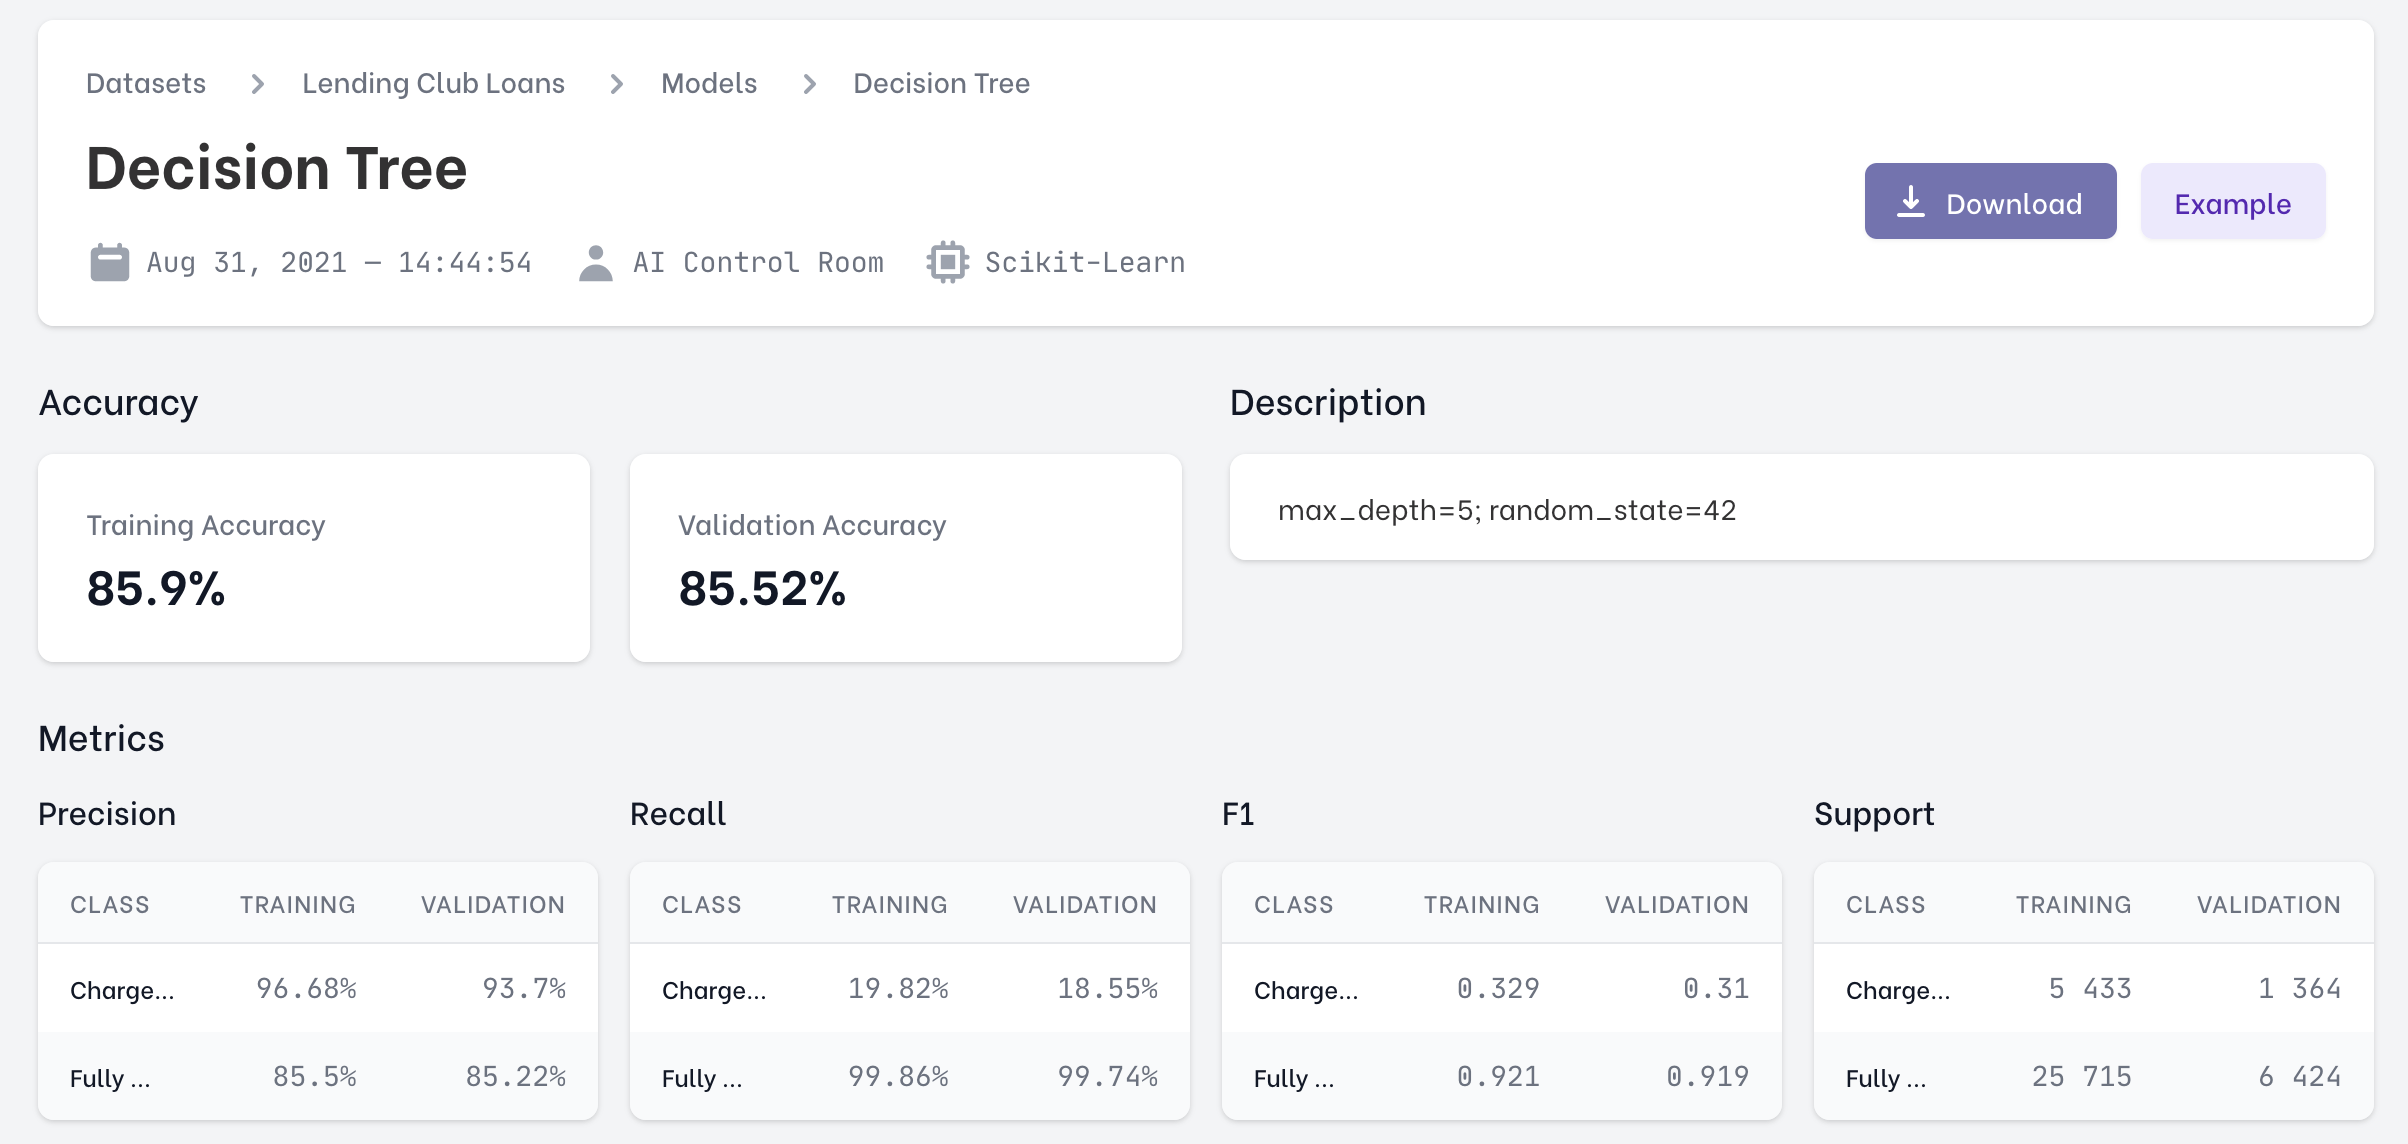
\includegraphics[width=\textwidth]{img/screenshots/model_assessment_overview.png}
    \caption{AI Control Room - Model Assessment Overview with Standard Metrics}
    \label{fig:model_assessment_overview}
\end{figure}
\begin{figure}[htbp]
    \centering
    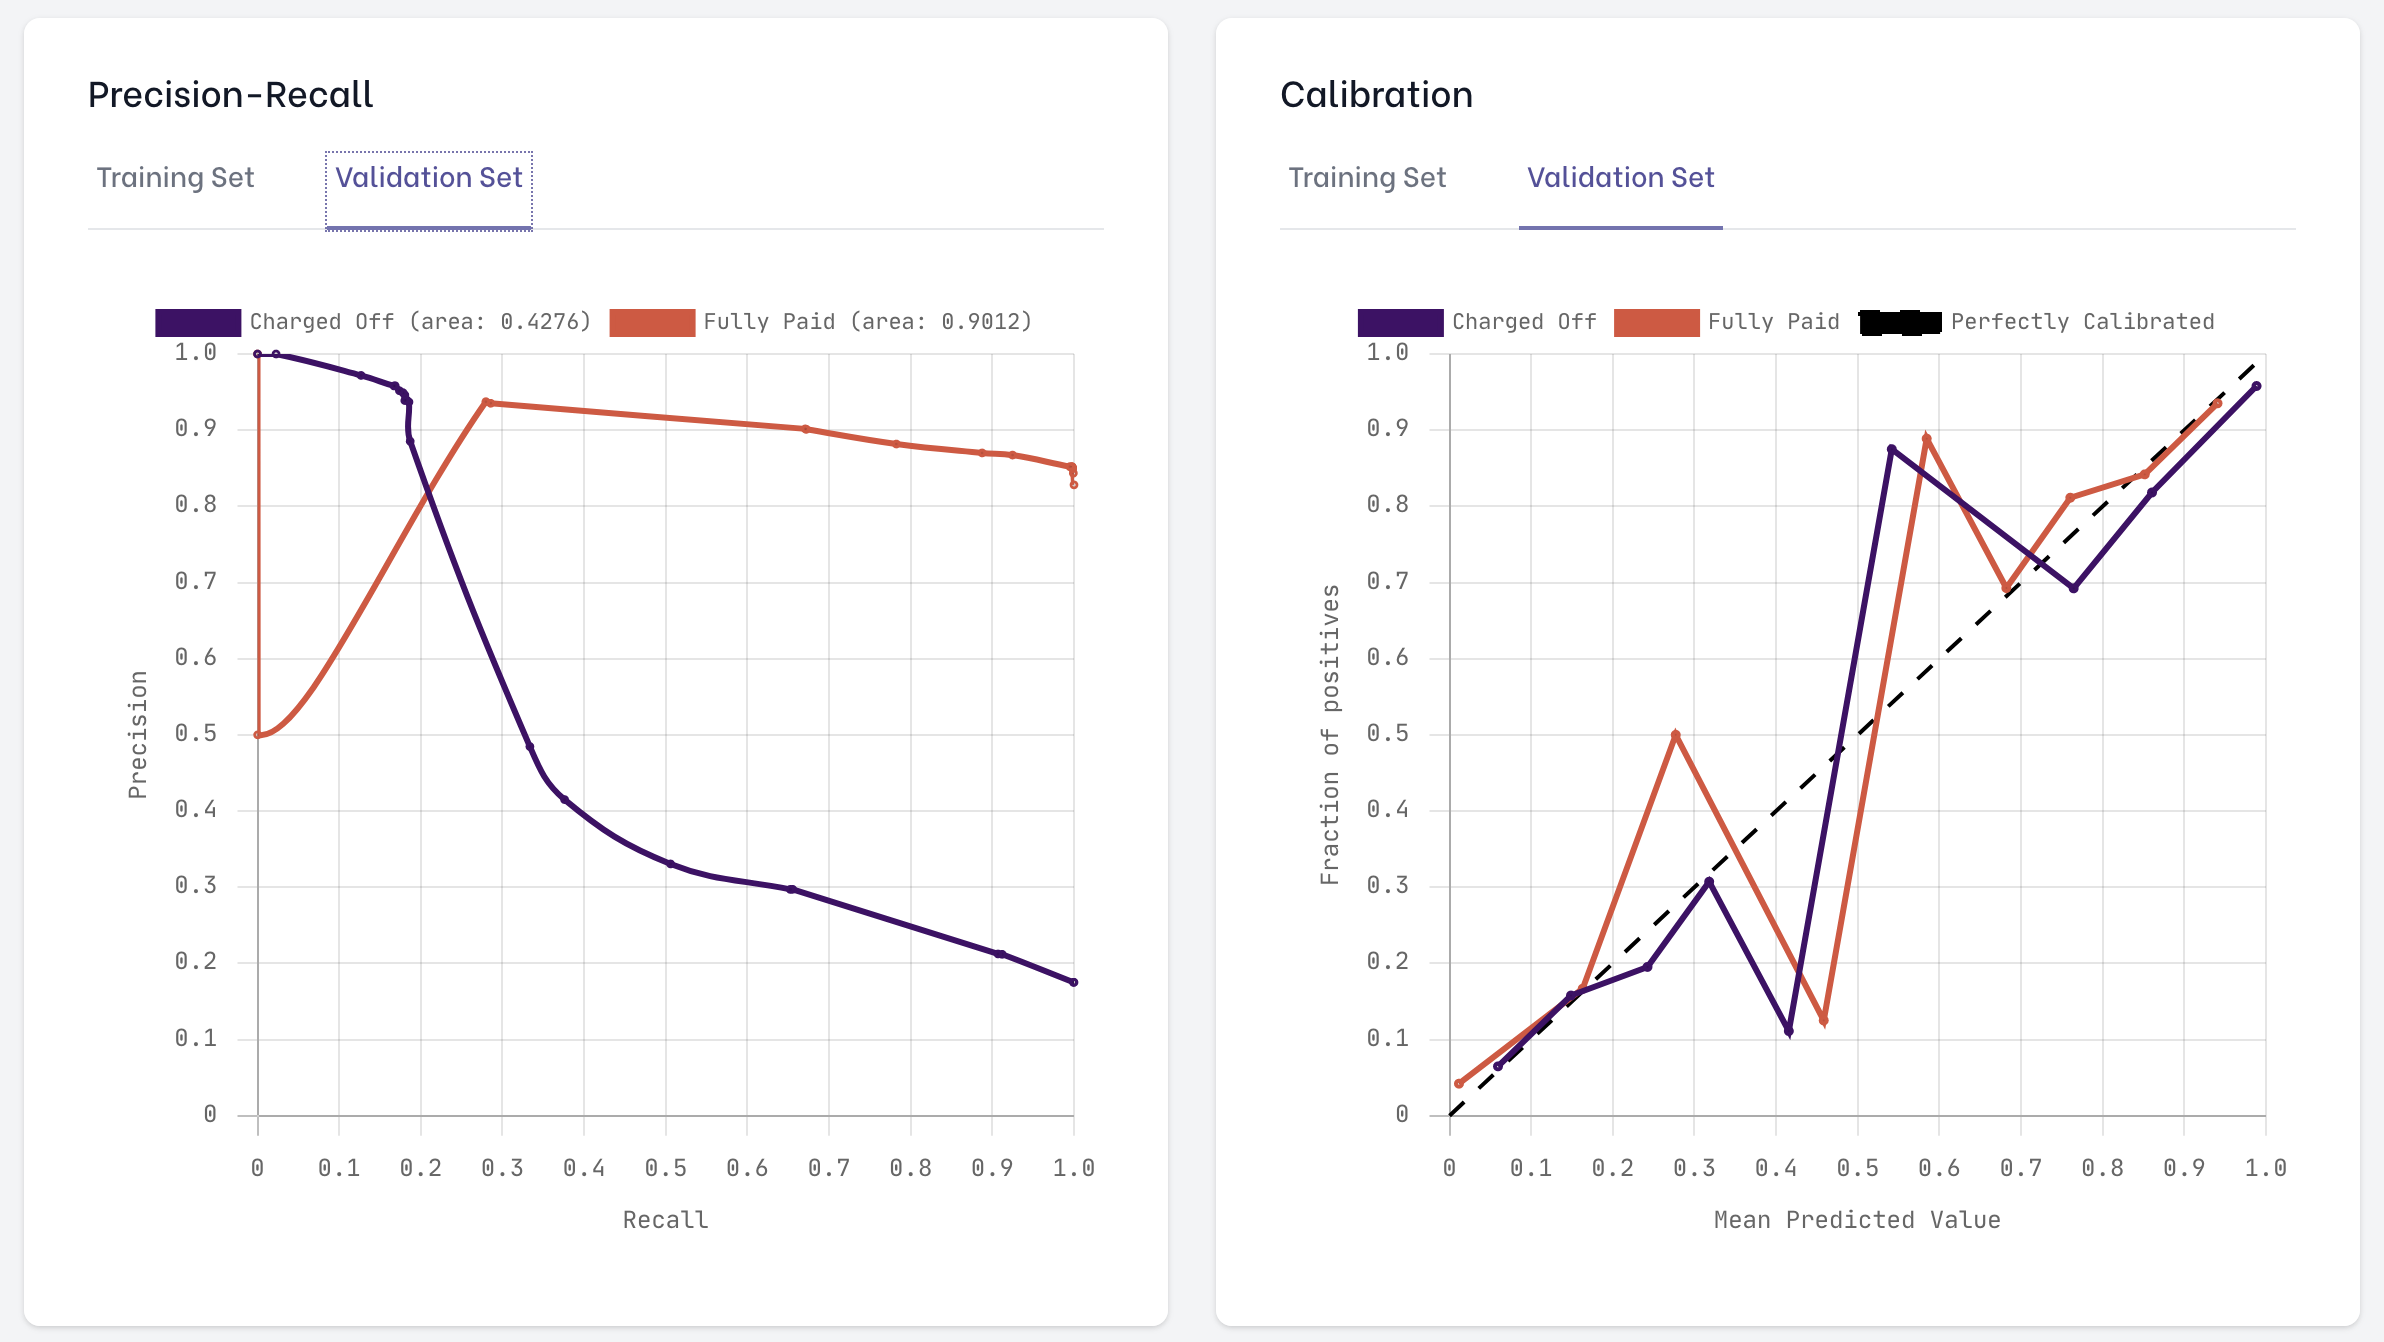
\includegraphics[width=\textwidth]{img/screenshots/model_assessment_graphs.png}
    \caption{AI Control Room - Precision-Recall and Calibration Graphs}
    \label{fig:model_assessment_graphs}
\end{figure}
\begin{figure}[htbp]
    \centering
    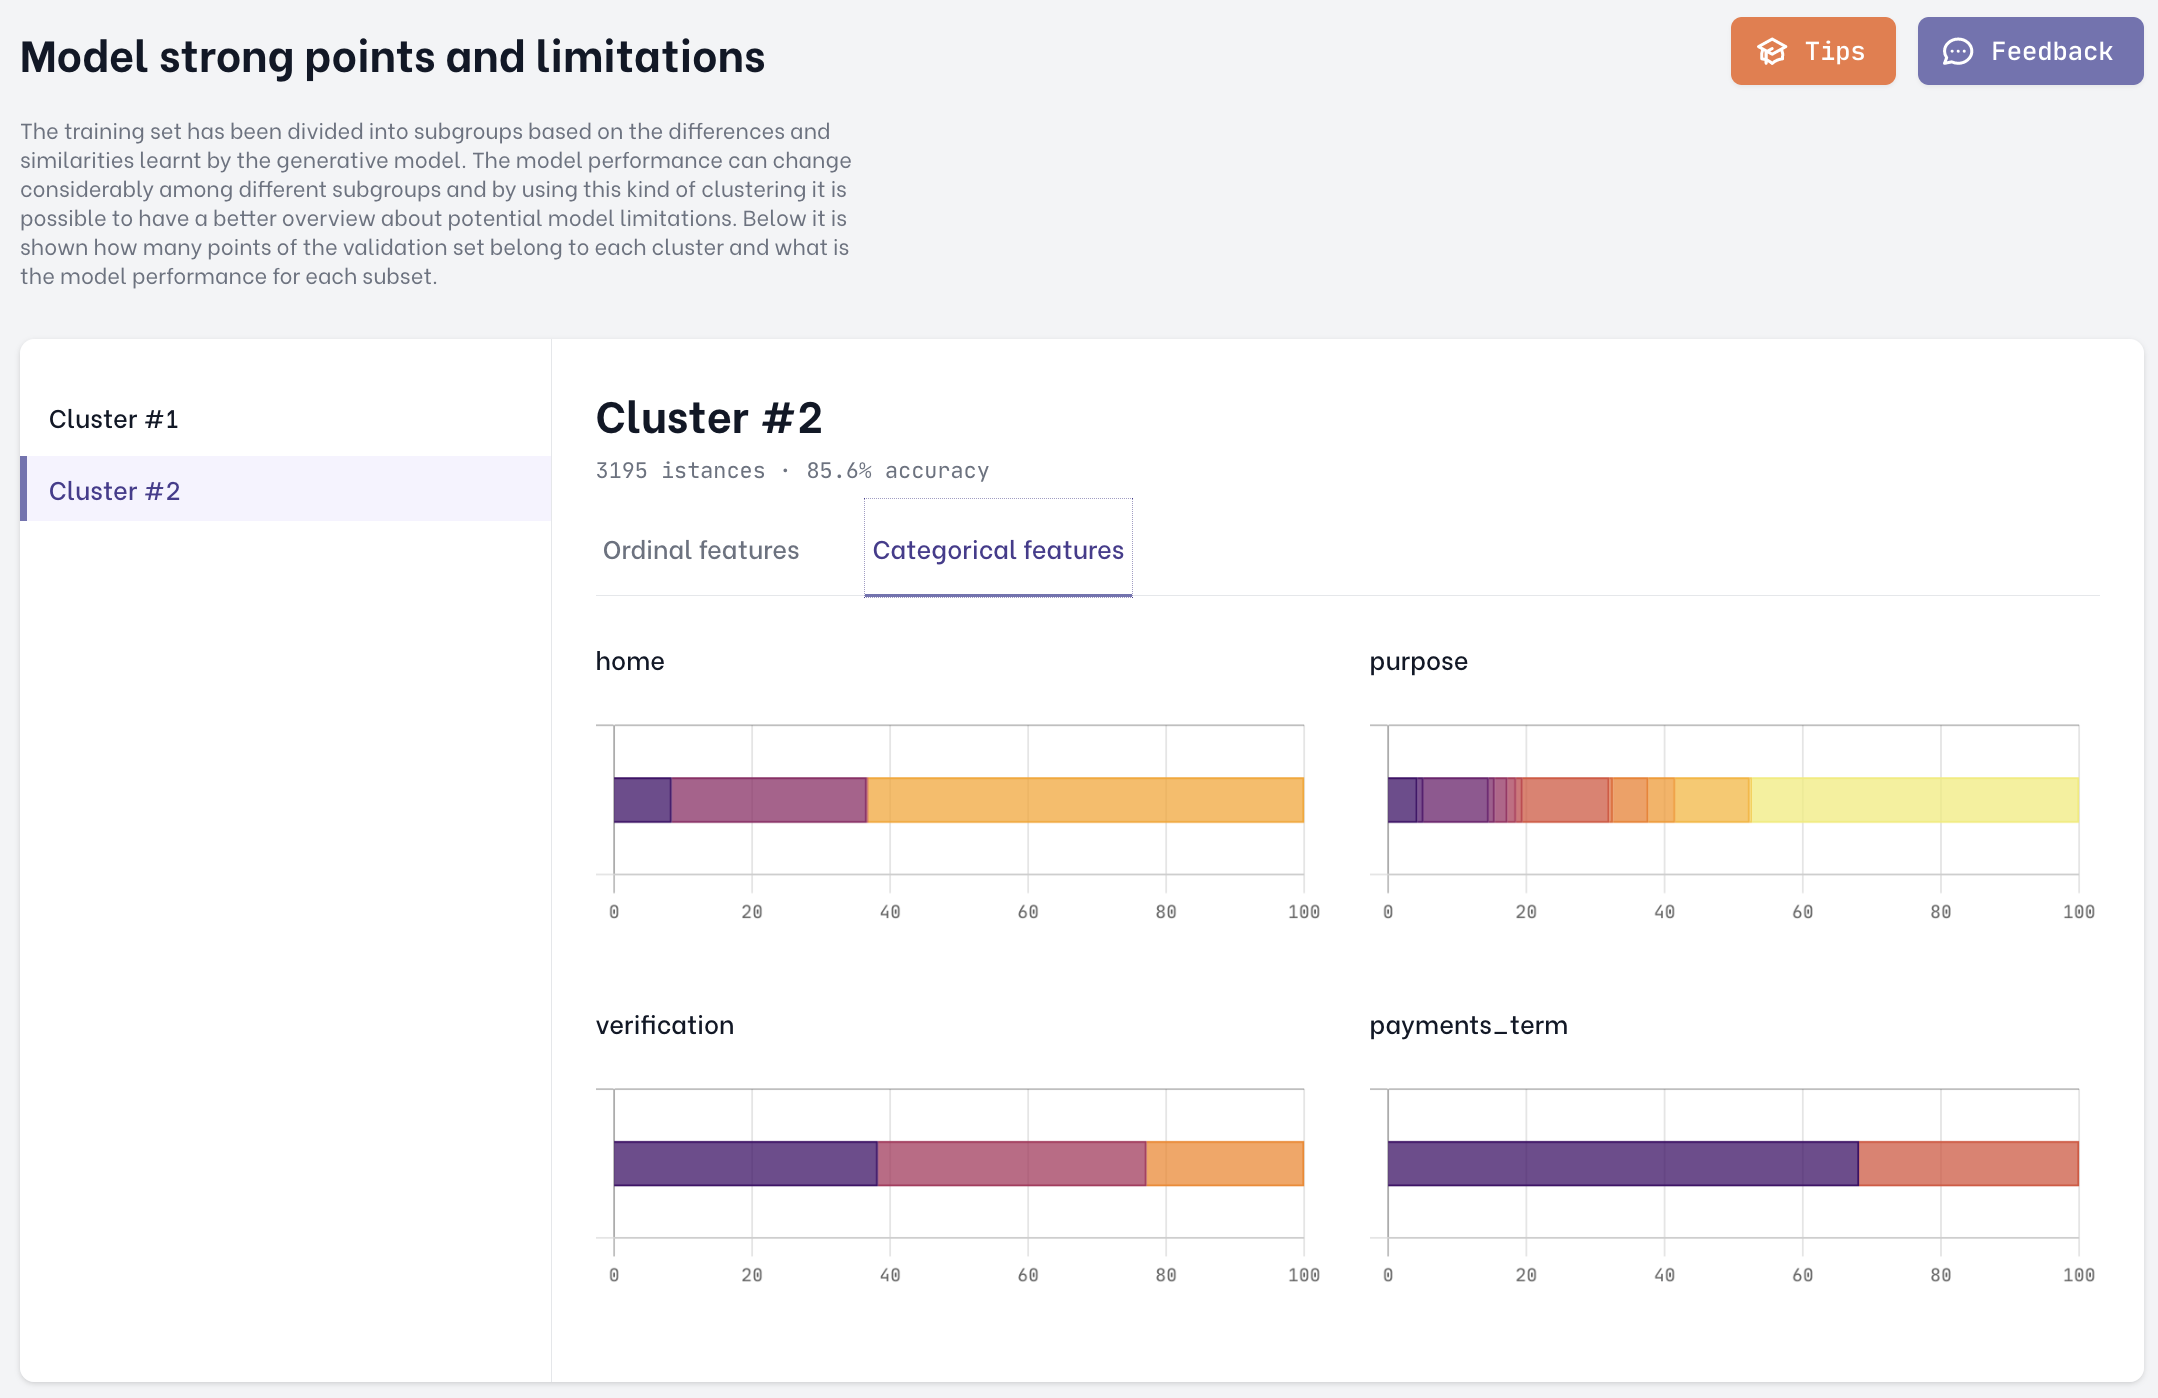
\includegraphics[width=\textwidth]{img/screenshots/model_assessment_analysis.png}
    \caption{AI Control Room - Model String Points and Limitations}
    \label{fig:model_assessment_analysis}
\end{figure}
\begin{figure}[htbp]
    \centering
    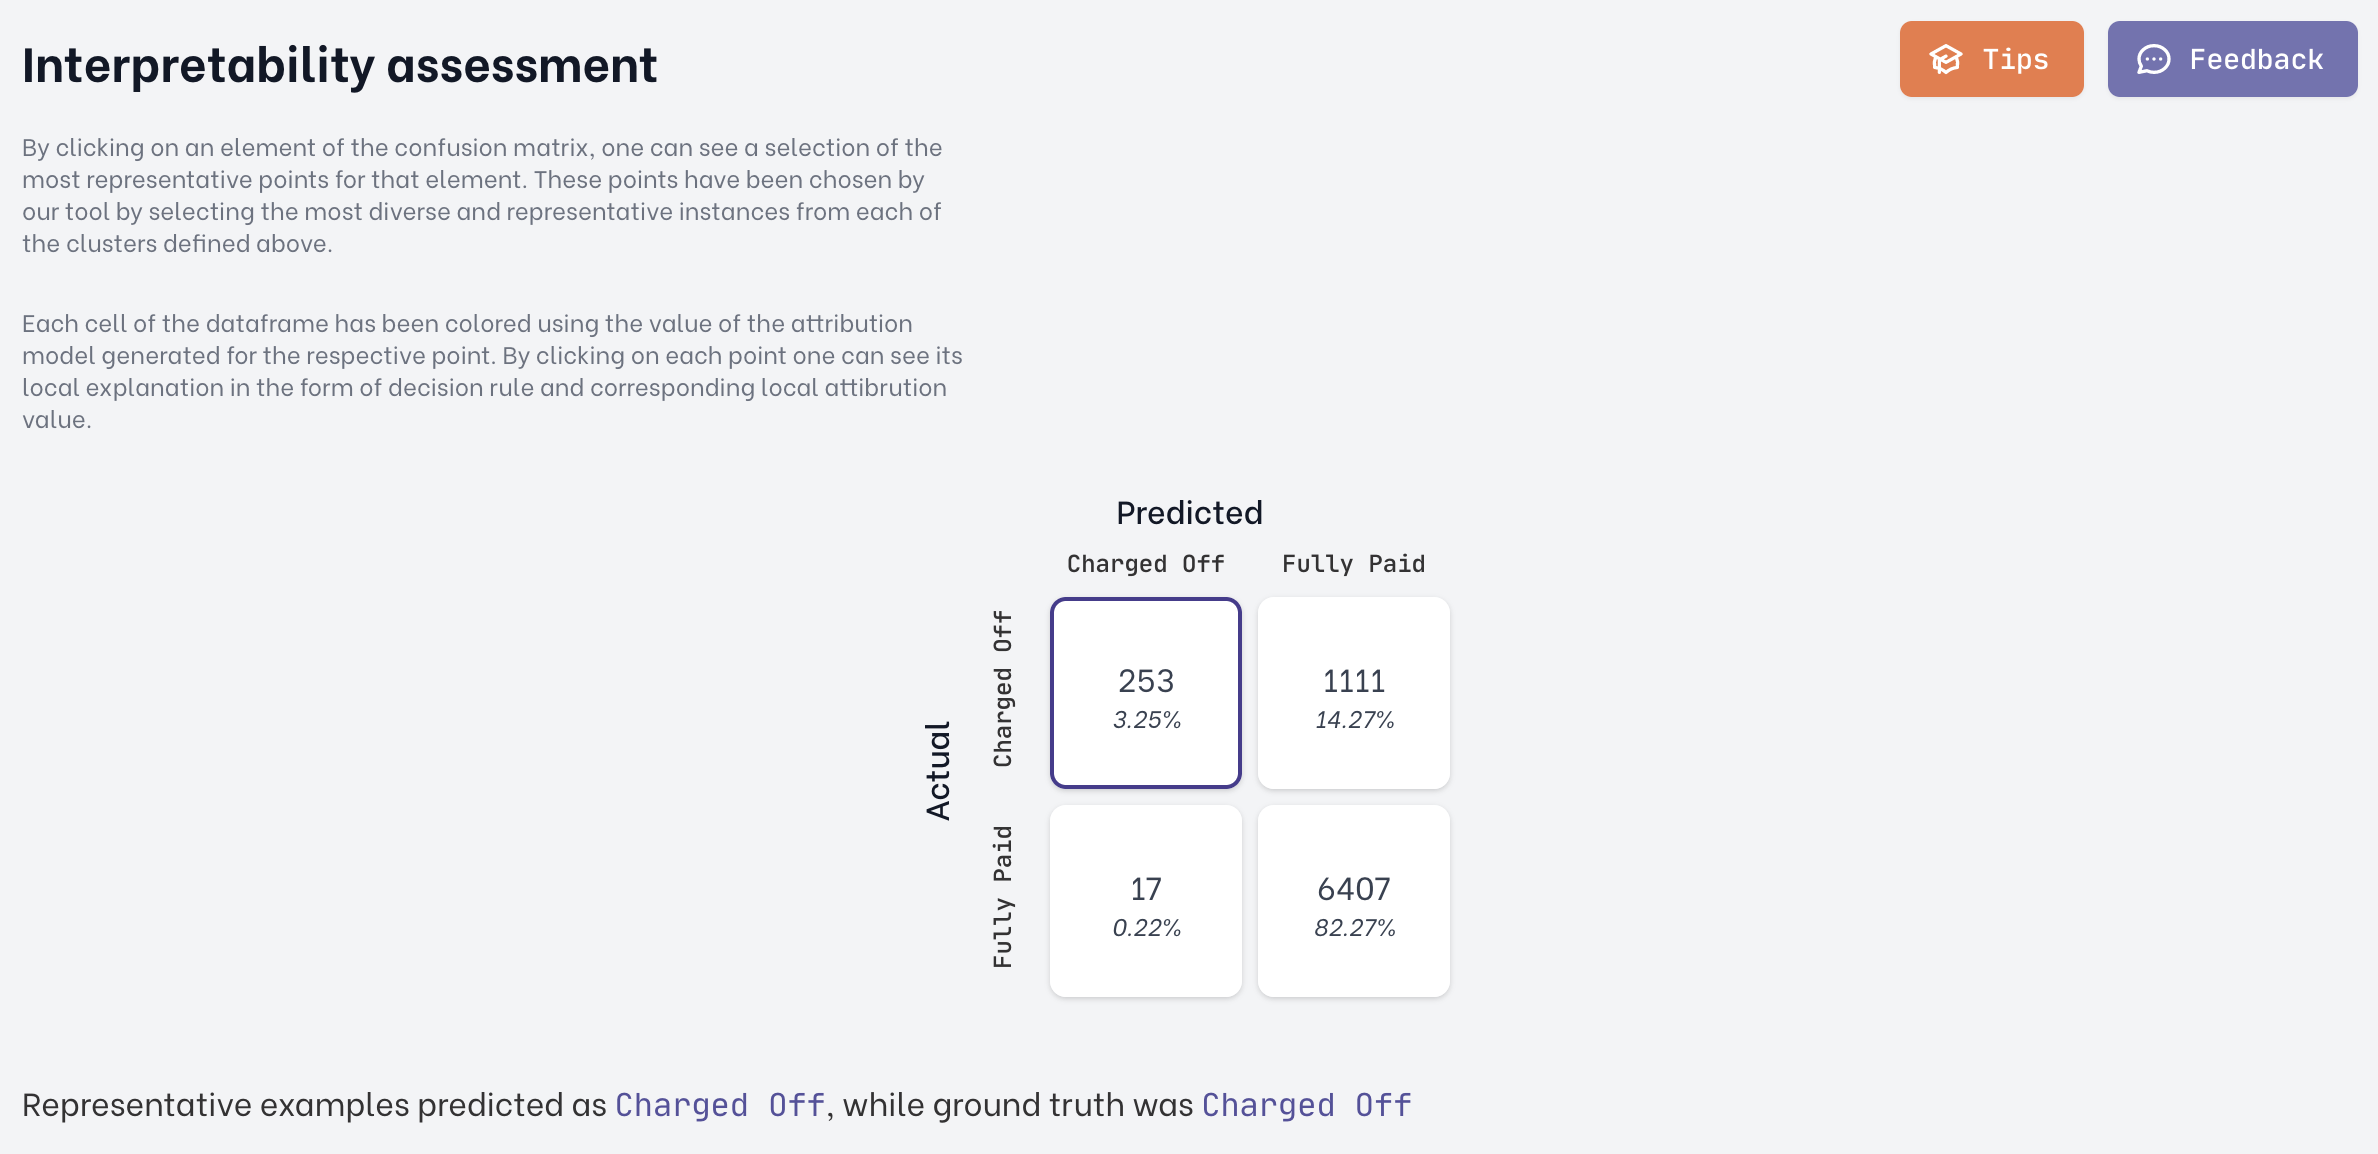
\includegraphics[width=\textwidth]{img/screenshots/model_assessment_interpret.png}
    \caption{AI Control Room - Interpretability Assessment}
    \label{fig:model_assessment_interpret}
\end{figure}
\begin{figure}[htbp]
    \centering
    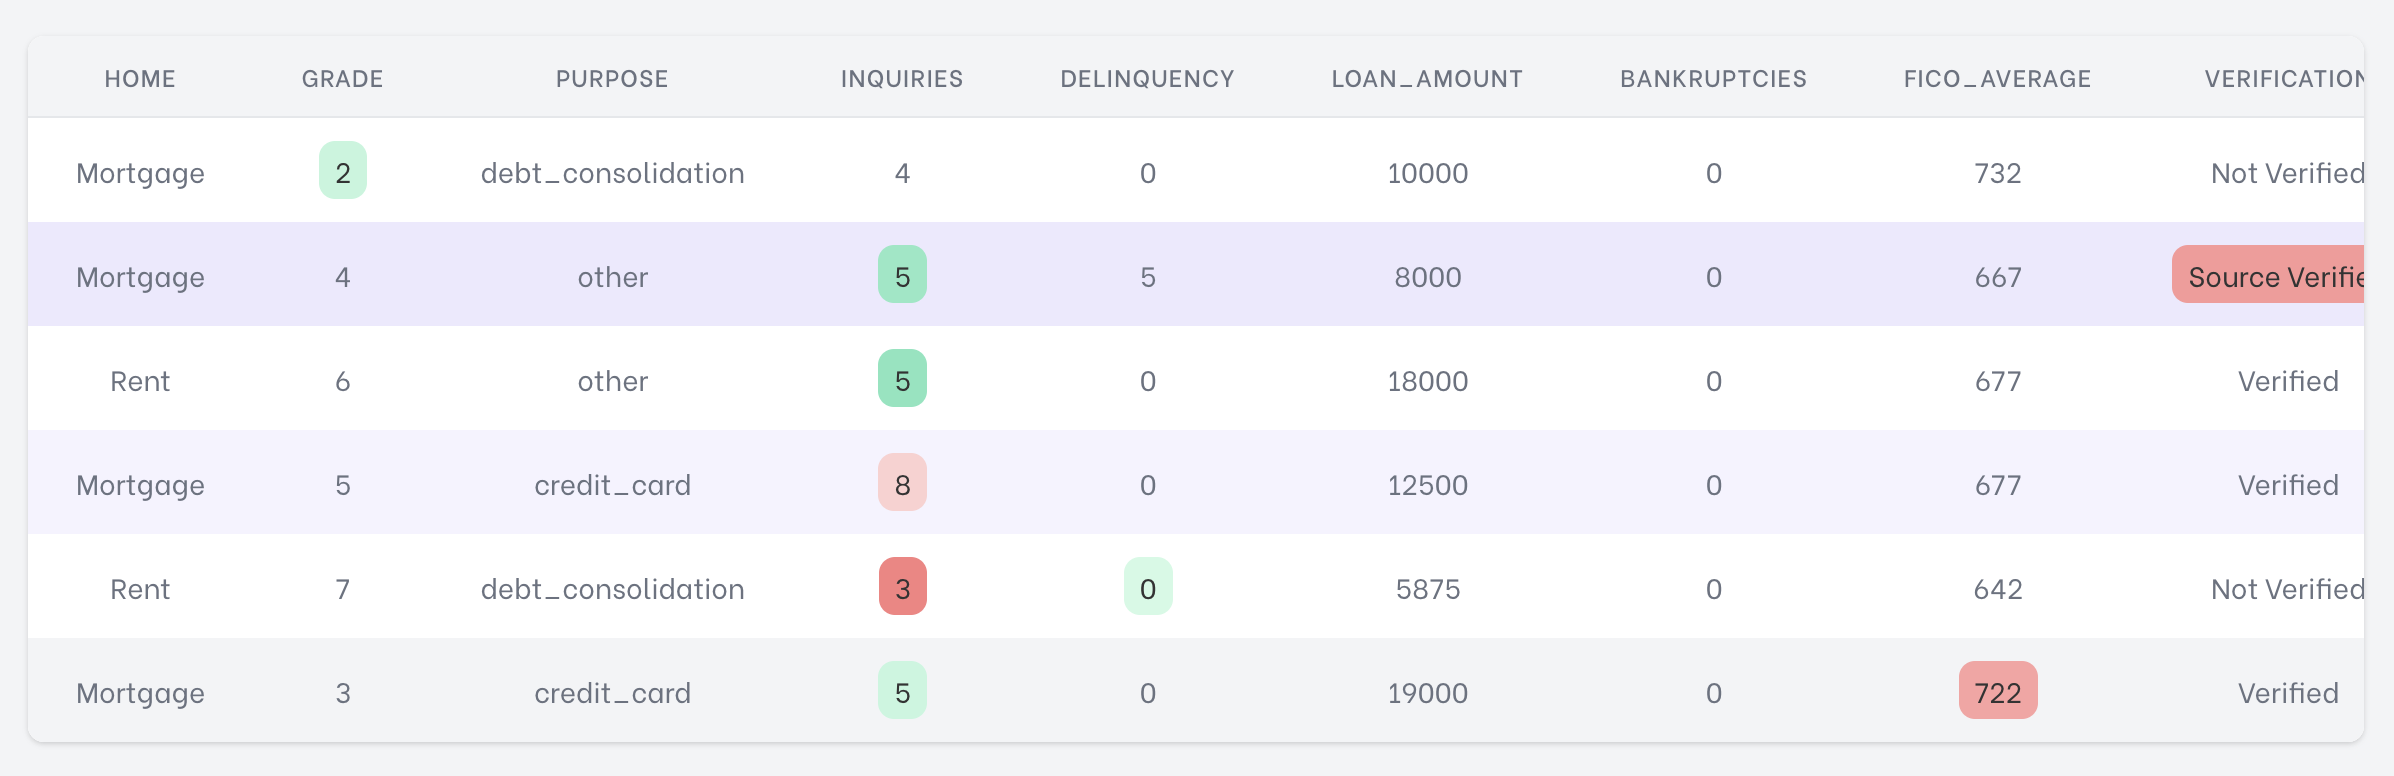
\includegraphics[width=\textwidth]{img/screenshots/model_assessment_examples.png}
    \caption{AI Control Room - Example Data}
    \label{fig:model_assessment_examples}
\end{figure}
\begin{figure}[htbp]
    \centering
    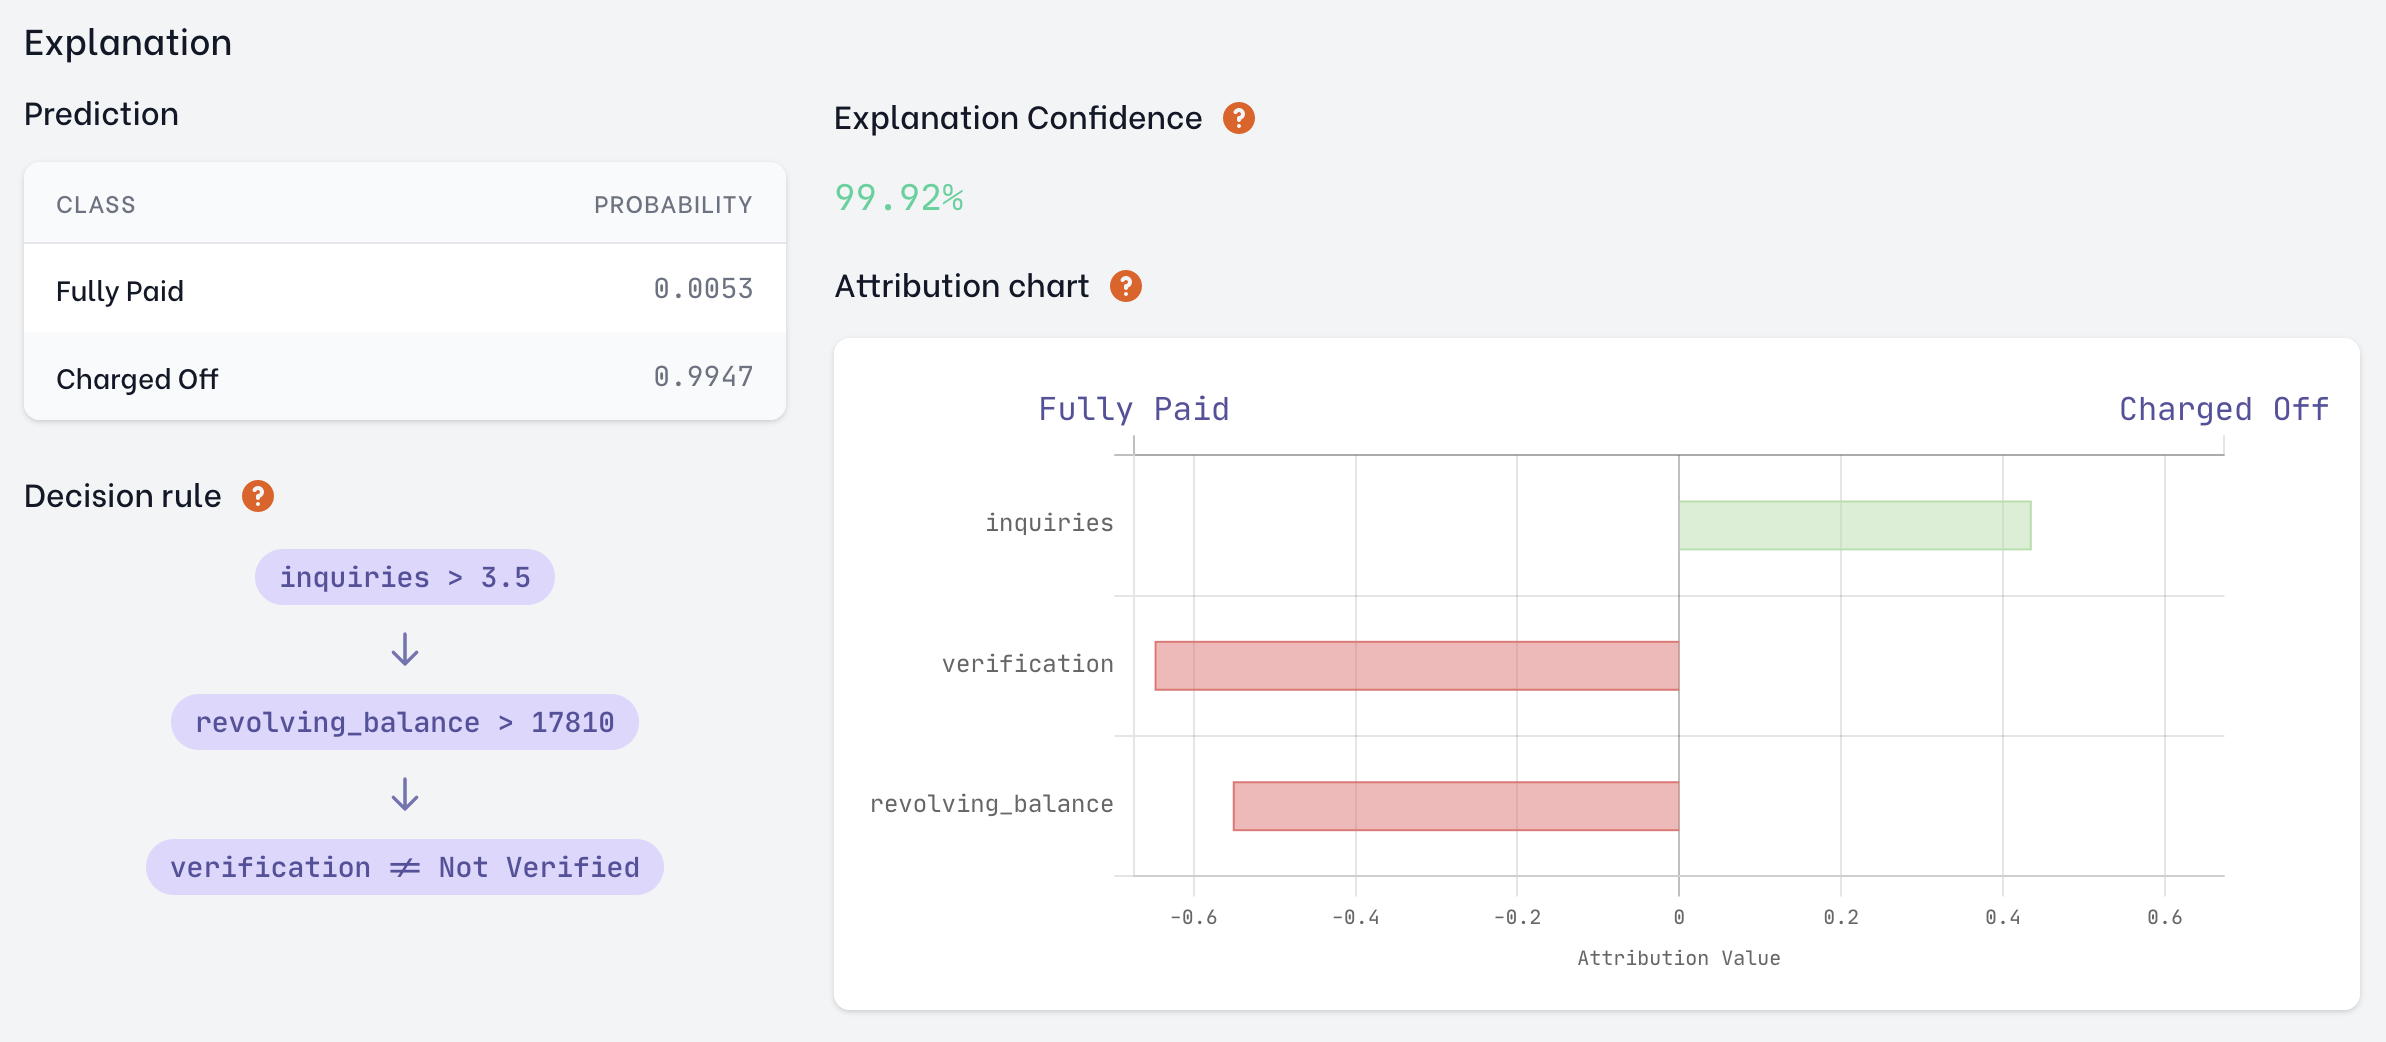
\includegraphics[width=\textwidth]{img/screenshots/model_assessment_explanation.png}
    \caption{AI Control Room - Prediction Explanation for Examples Data}
    \label{fig:model_assessment_explanation}
\end{figure}
\clearpage

\section{Approach}
As already described in the introduction of \autoref{chapter:introduction}, many machine learning algorithms score high on standard performance metrics, but user-facing performance may be way worse \parencite{gordon_disagreement_2021}. This issue is caused by real world applications being very dependent on the actual human-AI-interaction. Following this reasoning, it lends itself to utilize a human-centered design process for creating AI-assessment systems. \autoref{fig:DIN_EN_ISO_9241} shows a standardized process of human-centered design, which was applied in this thesis to conceptualize, implement and evaluate assessment system artifacts. The key take-away is the inclusion of human aspects in all stages of the process. Research on evaluation of AI explanations revealed that there is a big gap between the perceived and actual usefulness of explanations, as described by \textcite{ras_explainable_2021}. This further underlines the need for a human-centered approach in designing AI-assessment-systems.

The thesis' structure will reflect the human-centered approach, which is visualized in \autoref{fig:DIN_EN_ISO_9241}: As already alluded in \autoref{chapter:introduction}, \autoref{chapter:analysis} is about understanding and setting the context of use by conducting literature research and user interviews. Based on the established requirements \autoref{chapter:conception} will describe the conception of functionalities and interaction design. The development of solutions will be described in \autoref{chapter:implementation}, while \autoref{chapter:evaluation} is about the evaluation of the solutions. This general process is embedded in a iterative loop, where intermediate results are evaluated against the requirements and subject to change.
\begin{figure}[htbp]
    \centering
    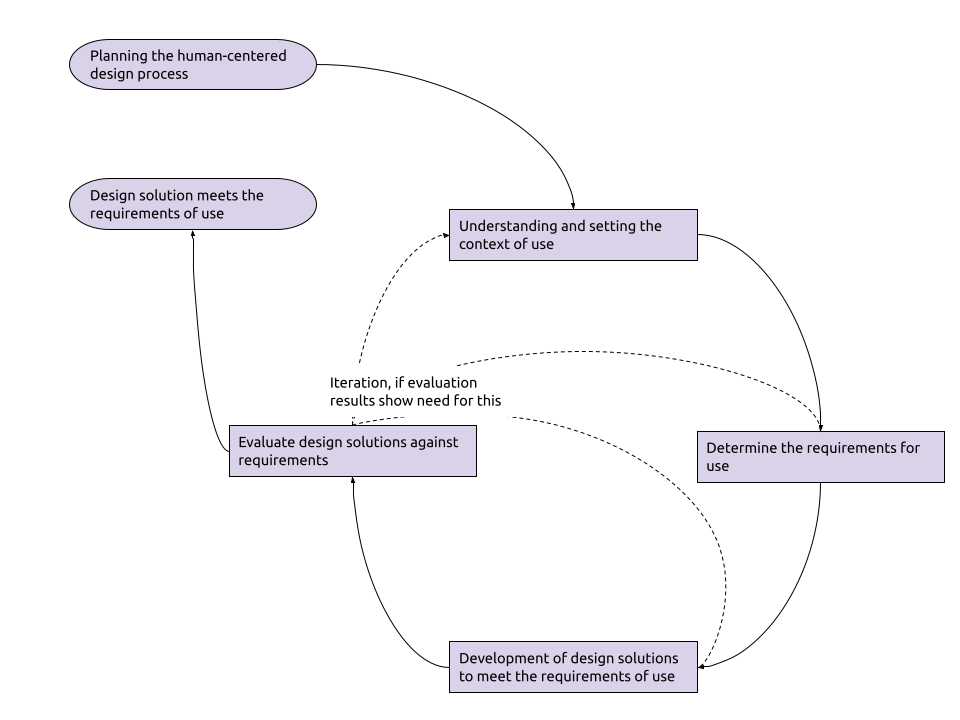
\includegraphics[width=\textwidth]{img/figures/DIN_EN_ISO_9241-210.png}
    \caption{Human-centered Design Process \parencite{DIN}}
    \label{fig:DIN_EN_ISO_9241}
\end{figure}

\newpage
\chapter{Analysis}\label{chapter:analysis}
Following the human-centered design process, it is important to incorporate the potential users from the beginning. This is also reflected in the analysis, where the context and setting of use has to be understood and set. Besides the human factors, there are also more general and theoretical aspects to be analysed, such as the context of AI in the medical application domain for specific tasks, such as classifying disease patterns with medical imaging.

In the following the context, task, problem and users will be described and analysed as a foundation for the human-centered design process and the following conception of AI assessment system artifacts.

\section{Data Sources}
Three main data sources where used for the analysis, ranging from general scientific literature about XAI to specially elaborated user interviews and cooperation with developers of an existing application.

\subsection{Scientific Literature}
Literature is the foundation of the analysis. As described by \textcite{mueller_explanation_2019}, the amount of scientific publications on the topic of explanation in intelligent systems has surged in the last 5 years, revealing many important and relevant information on this subject area through openly accessible papers. In the beginning of the thesis (July 2021) a general search on \textit{Google Scholar} was conducted to gain a overview on available publications. A non-exhaustive list of search terms at the time was:
\begin{itemize}
    \item XAI
    \item XAI in Medical Applications
    \item Explainable Artificial Intelligence
    \item Explainable Artificial Intelligence in Medical Applications
    \item Explainable Machine Learning
    \item Interpretable Machine Learning
    \item Explaining Black-Box Machine Learning Models
    \item Explaining DNNs
\end{itemize}
This general research yielded already good results, as there were many relatively new and popular publications on the topic of XAI, such as \textcite{mueller_explanation_2019, ras_explanation_2018, adadi_blackbox_2018, hoffman_metrics_2019}.

The results of the internet research were then further reinforced by academic partners from the University of Lübeck, with whom related research was conducted in the context of the \textit{CoCoAI} project. Leveraging the available resources and support from research partners boosted the yield on relevant scientific literature tenfold. Over the course of multiple months the list of literature grew and is still being maintained in a shared \textit{Zotero} library \parencite{zotero_website}. The most important scientific papers for this analysis were: \textcite{ras_explanation_2018, arrieta_explainable_2019, ribeiro_why_2016, adadi_blackbox_2018,knapic_explainable_2021, samek_explaining_2021, chiou_trusting_2021, hoffman_metrics_2019}. 

\subsection{Interviews}\label{subsection:interviews}
Complementing the general research on XAI, specially elaborated user interviews where conducted. These interviews specifically target medical professionals and data scientists. Interviews with the actual user group of a potential solution is key to understanding and setting the context and requirements of use. The participants for the interviews were chosen with following requirements in mind:
\begin{description}
    \item[Medical Professionals:] Has interest and/or knowledge in AI-systems; has worked with or researched AI-systems in the medical domain; can judge the benefits and risks of the use of AI in medical applications.
    \item[Data Scientists / AI Researchers:] Is familiar with the XAI topic; has interest in explainability and trustworthiness of machine learning models; has worked with AI in the medical context.
\end{description}
Participants for the interviews were gathered via academic partners, internet research and word of mouth. In total 16 suitable people from 6 different institutions (among them UKSH, TU München and Mevis Frauenhofer Bremen) were contacted about potential interviews. Ten leads were medical professionals while six leads where data scientists or AI researchers. From the total of 16 potential interview partners only four interviews have been conducted. This low yield is due to the time constraint of the individuals, who are mainly full time medical practitioners or researchers. The participants are described in further detail in \autoref{table:interview_participants}.

\begin{table}[htbp]
    \centering
    \begin{tabularx}{\textwidth}{ l l l X X l }
        \toprule
        ID & Age & Gender & Occupation & Education Level & AAII Score \\
        \midrule
        1 & 28 & male & Assistant Physician in Neuroradiology & State Examination & 4.89 \\ 
        2 & 24 & female & Research Associate (ML) & Masters Degree & 5.12 \\ 
        3 & 48 & male & Surgeon & Dr. med. & 5.45 \\ 
        4 & 27 & female & Assistant Physician in Neuroradiology & State Examination & 4.67 \\ 
        \bottomrule
    \end{tabularx}
    \caption{Interview Participants}
    \label{table:interview_participants}
\end{table}

The Interviews were conducted in german and executed as 1 to 1 online interviews. For reference the interviews were recorded if consent was present. Additionally the interviews were supported by a research colleague, who kept protocol. After the interviews the recordings were transcribed for further analysis and the participants were asked to answer the \textit{Affinity for AI Interaction} (\textbf{AAII}) questionnaire, which is a modified version of the \textit{Affinity for Technology Interaction} (\textbf{ATI}) questionnaire \parencite{franke_personal_2019}. ATI aims to determine the tendency to actively engage in intensive technology interaction, as a key personal resource for coping with technology. Analogously the AAII questionnaire aims to determine the tendency to actively engage in AI interaction.

In terms of content, the interviews for medical professionals and data scientists were slightly different as seen in \autoref{table:interview_topics}. The reason for this is the heterogenous expertise on the subject area of machine learning models and potential user requirements. The whole interview guideline can be found in \autoref{appendix:interview_guideline}.
\begin{table}[htbp]
    \centering
    \begin{tabularx}{\textwidth}{ l l }
        \toprule
        Medical Professionals & Data Scientists / AI researchers \\
        \midrule
        Actual Usage of AI & Actual Usage of AI \\ 
        Perspective on AI Usage & Comparison of AI Models \\  
        Trust in AI & Perspective on AI Usage \\
        Potential Problems with AI Usage & Trust in AI \\
        Own Explanation Techniques & Potential Problems with AI Usage \\
        Familiarity with XAI & Own Explanation Techniques \\
        Assessment on Local Explanations & Familiarity with XAI \\
        Information Processing & Need for Local Explanations \\
        Reliability vs. Trust vs. Understanding & Need for Global Explanations \\
         & Information Processing \\
         & Trust-Behavior Connection \\
         & Reliability vs. Trust vs. Understanding \\
        \bottomrule
    \end{tabularx}
    \caption{Interview Topics}
    \label{table:interview_topics}
\end{table}

After gathering the interview data via protocols and transcripts a thematic analysis according to \textcite{braun_thematical_2006} was applied to identify common topics and codes. The thematic analysis is a widely used qualitative analysis method mainly found in the field of psychology and can be used as a primary tool to access data from interviews. Applying this method resulted in a thematic map showcasing common overlapping topics found in the interviews, which can be seen in \autoref{fig:thematic_mind_map}. The thematic map serves as the baseline for further context and requirement analysis.

\begin{figure}[htbp]
    \centering
    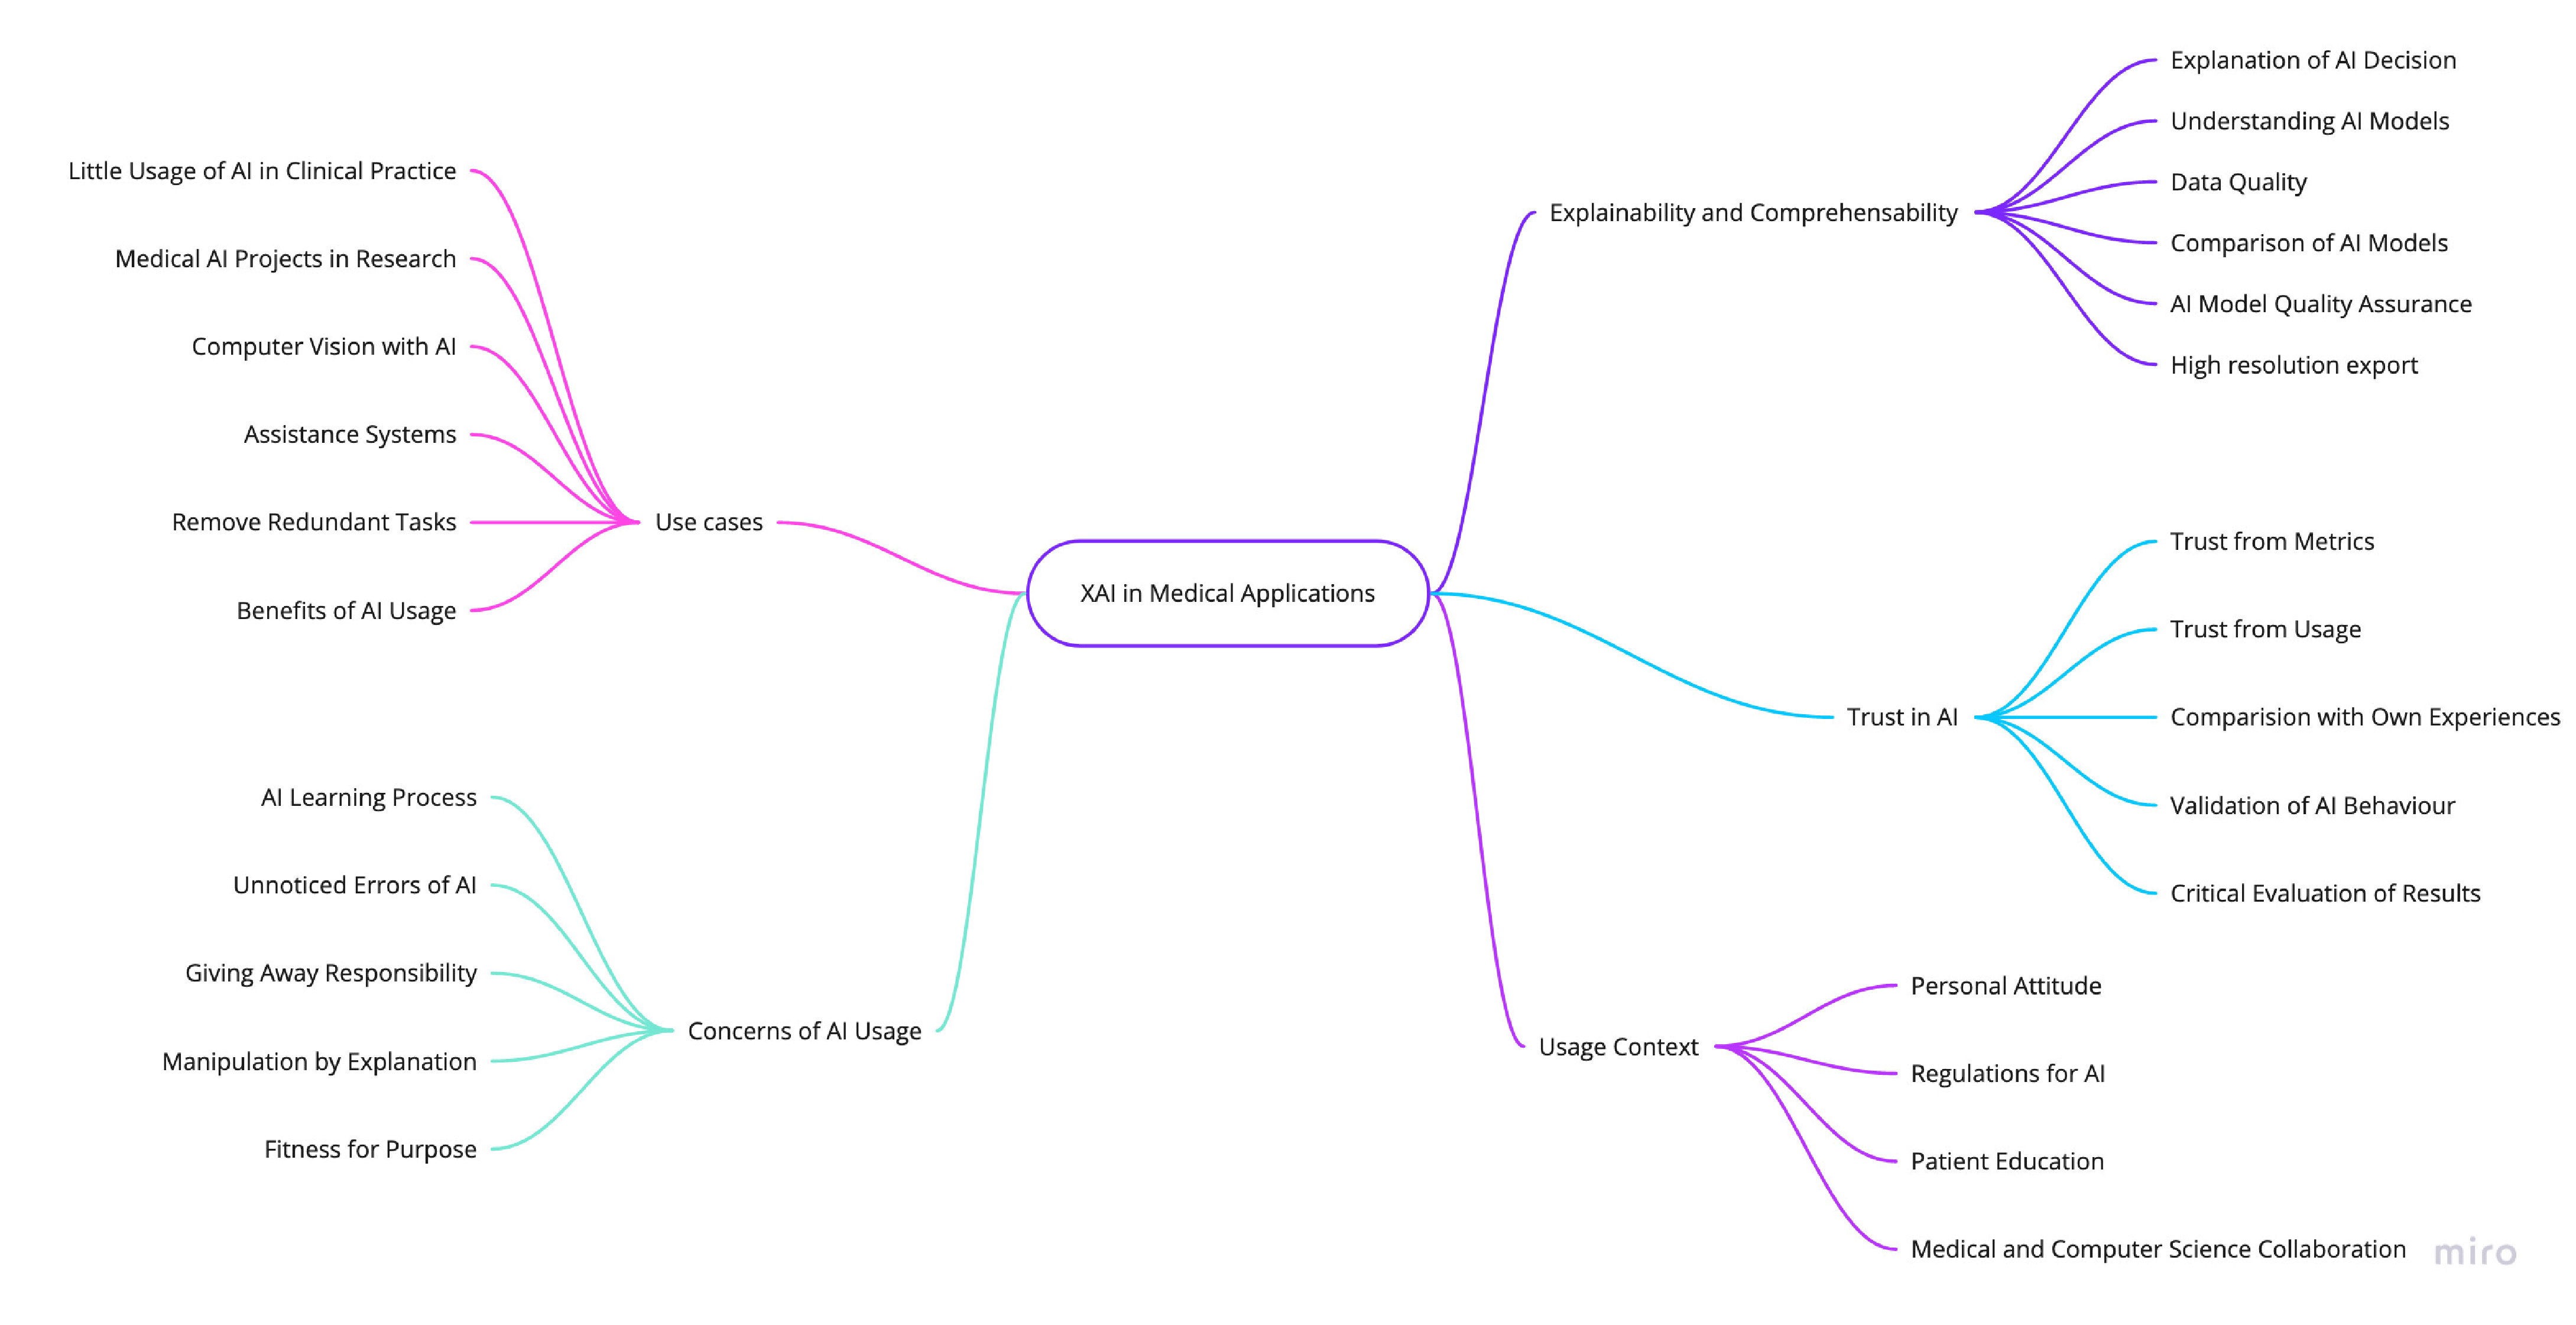
\includegraphics[height=0.8\textwidth, angle=90]{img/figures/Thematic_Mind_Map.pdf}
    \caption{Thematic Mind Map}
    \label{fig:thematic_mind_map}
\end{figure}

\subsection{Existing Applications}\label{subsection:existing_apps}
A scientific cooperation with Clearbox AI allowed us to access a additional source of information, valuable for the analysis and conception. As already described in \autoref{section:state_of_the_art} Clearbox developed an AI model assessment solution among other things. During the period of cooperation regular meetings were held with the CTO and other employees. These meetings were used for knowledge exchange on the subject of XAI literature, previous experiences, feedback and conceptional workshops.

The enormous previous experience of Clearbox is a great resource of information for the thesis. Many aspects of analysis and conception were supported by the regular, bi-weekly meetings. In particular, resources such as \textcite{people_ai_google_website, captum_website,streamlit_website, lapuschkin_unmasking_2019} were supplied by Clearbox. Furthermore the (beta) access to the Clearbox AI \textit{Control Room} cloud platform and the communication of user feedback was invaluable to gather information on the analysis and conception of an assessment system for image-based AI models.

\section{Context Analysis}
Black-box DNNs have become pervasive in todays society and represent a proven and indispensible machine learning tool. While these machine learning models can easily be used in recreational non-risky contexts, this does not hold true for the medical domain where decisions based on the results of a machine learning model can bear great risks for users and patients. This issue stems from the lack of interpretability and trustworthiness of DNNs \parencite{adadi_blackbox_2018}. DNNs architectures are inherently hard to understand and therefore interpretability of and trust in the results of such neural networks are a challenge.

Creating a solution to explain AI models a priori to the use can help setting the right expectations towards the AI model. Consequently the users of such a explanatory system gain the ability to build a fair mental model before using the AI, which in turn can support the formation of appropriate levels of trust \parencite{hoffman_metrics_2019}. This is beneficial to the user and facilitates efficient usage of the model in production \parencite{hoffman_metrics_2019, people_ai_google_website}.

Explaining the model a priori also enables the solution to build computationally complex explanations, which can depend on datasets of thousands of images. Supplying the user with explanations potentially based on the whole dataset can also be beneficial: Statistical analysis and clustering of the data and metadata can support the understanding of model limitations and edge cases, while exemplary local explanations can be statistically distributed to gain a better overview of global behavior of the model. Combining different types of a priori explanations improve the coverage of the key attributes of explanations - understandability, feeling of satisfaction, sufficiency of detail, completeness, usefulness, accuracy, and trustworthiness - which were described by \textcite{hoffman_metrics_2019}.

The aspects mentioned above are also reflected in the interview data. The following list showcases translated quotes from interview partners regarding the need for (a priori) explanations for AI models aimed at the medical domain:
\begin{displayquote}
    "I think you have to be critical and look at the results carefully - is the result at all plausible?"
\end{displayquote}
\begin{displayquote}
    "What is the information that is interesting for the system or that is decisive for the decisions? What information is rather irrelevant?"
\end{displayquote}
\begin{displayquote}
    "If the explanations for the model are based on any data that are meaningless from my clinical experience, such as a stroke being pinned down by bone shapes. That would shake my confidence in the machine, even though it might give reliable results."
\end{displayquote}
\begin{displayquote}
    "If, for example, there is an outlier data point in a specific case and you are not quite sure why it is like this or how you should interpret it, then something like this [local explanation] is great, so that you can understand why the result is like this or like this."
\end{displayquote}
\begin{displayquote}
    "I've always been interested in exactly how this works, how much training data it's based on, what's behind it, why the system decides the way it does."
\end{displayquote}
\begin{displayquote}
    "[...] and you might also learn what the machine pays attention to, which I personally could also pay attention to when I look at the picture. That would certainly strengthen my confidence in the application."
\end{displayquote}

\section{Problem and Task Analysis}
The following problem scenario summarizes the starting point of the problem and task analysis: The general medical practitioner Dr. med. Mustermann wants to offer thrombosis diagnosis in his office. He is not specialized in vein examination and thus has just basic knowledge and also no necessary equipment. In the past this has lead to him referring patients with venous disorders to a specialized clinic. Through a colleague he was made aware of "\textit{AutoDVT}", a AI-based software developed by ThinkSono, which can help him offer DVT diagnosis in his office. The AutoDVT system works with image-based machine learning and can support medical professionals in real time with identifying DVT. Since Dr. med. Mustermann has very little knowledge of AI and machine learning he is very skeptical towards this innovative but foreign software system. Although he sees the immediate benefits of using a system which supports him with the examination of DVT, his trust in the system’s predictions is very low and he fears relying on the AI’s assessment. AI-based technology is a black box for him, which he does not fully understand. The predictions of the systems are opaque to him and thus lead to rejection of the system.

DNNs for image classification are able to detect various disease patterns with medical imaging and can be used by medical professionals to support diagnosis and possibly increase efficiency and effectivity if trusted and used correctly \parencite{adadi_blackbox_2018,knapic_explainable_2021}. However, the reality looks different: Medical professionals bear the responsibility for their decisions regarding the patient and thus are rather relucant about using AI based systems - even though the AI could outperform them in image classification tasks. Most of the time decisions are based on personal experience, which was developed over a long period of time. This sentiment is reflected in the interview statements of medical professionals:
\begin{displayquote}
    "One risk, I believe, is also that you hand over responsibility to the machine."
\end{displayquote}
\begin{displayquote}
    "The classic risk of simply relying on what the algorithm says."
\end{displayquote}
\begin{displayquote}
    "The doctor with his expert knowledge will always compare this with his knowledge and experience, is this correct, what is the probability, is this in the range?"
\end{displayquote}

Modern DNN based image classificators, such as the \texttt{XRV\--DenseNet121\--densenet121\--res224\--all} model from \textcite{cohen_limits_2020}, can provide very good results in the prediction of pathologies. For example, the prediction accuracy for pneumonia is benchmarked as 86\% \parencite{torchxrayvision_github}. The use of such model or comparitive ones could benefit medical professionals in many ways as described by the interview partners:
\begin{displayquote}
    "It [AI system] facilitates standardized findings in particular"
\end{displayquote}
\begin{displayquote}
    "It [AI system] might give you a little peace of mind that you haven't missed anything."
\end{displayquote}
\begin{displayquote}
    "I always think to myself that this is based on CT gray levels, i.e. on these density values, and I always think to myself that it makes sense that a computer can distinguish these density levels better than my eyes."
\end{displayquote}

The benefits of using a DNN based image classificator to support medical professionals in detection and diagnosis of diseases are clear. For users to leverage these benefits trust in such a system must be given, which cannot be generated by mere accuracy metrics \parencite{samek_explaining_2021}. To overcome the hesitation of using AI in medical applications, a AI assessment system can be used to facilitate understanding of and trust in the algorithms. Stakeholders, such as practitioners or clinic managements, can use such a system to gain customized insights into the model and data prior to using it in everyday clinical practice.

\section{User Analysis}
Trustworthiness and explainability of AI models only makes sense considering the potential user groups. For an assessment system that aims to explain AI models in the medical domain those user groups are: (1) Medical professionals, such as practitioners and clinic managements and (2) data scientists and AI researchers developing AI models. Naturally those two groups differ greatly from each other. While medical professionals have great expertise in various fields of examination, diagnosis and communication of pathologies, they also are expected to have little knowledge in computer sciences and machine learning. Data scientists on the other hand do have great knowledge of computer sciences, machine learning and neural network architectures, but lack the concrete medical expertise. Following the human-centered process the needs, requirements and whishes in regard to an AI assessment system of those user groups were analysed, mainly referencing the interviews from \autoref{subsection:interviews} and the resulting thematic map (see \autoref{fig:thematic_mind_map}).

\subsection{Medical professionals}
The user group of medical professionals is a very heterogenous one, which is to be expected from a professional field with many different specializations. This was also found out in the interviews. Surveying practitioners of different ages showed, that especially the younger ones, working in neuroradiology, are open towards using AI in their daily routine or that they are already using it. Great initiative was shown by two assistant physicians, who also took courses on machine learning in the medical domain during their studies. Then again the older, but way more experienced surgeon has stated that he has much less contact with AI in clinical practice. All interviewed medical professionals showed interest in medical AI in research projects and were positive on the benefits of AI, especially computer vision tasks. The most cited benefits were the great ability of machine learning to identify pathologies in medical images, the take over of redundant tasks, the backup for diagnosis and the handling of computationally expensive tasks. The medical professionals were also wary and timid about using AI. This stance was stated to be mainly routed in the missing experience in using and trusting these systems. The black-box character of DNNs was stated to be a central issue: Not being able to re-trace the decisions of the AI and having to give away responsibility lead to trust and compliance issues, which was already stated by \textcite{ras_explainable_2021}. Depending on standard metrics was also stated to be insufficient, as the interviewed experts showed interest in the training data set and active comparison of the AI's results with their own experiences. While standard metrics, such as accuracy, sensitivity and specificity were important to the interviewees, the critical evaluation of the results and the validation of the behavior were whished for by every one of them.

As \autoref{table:interview_participants} shows, all interviewees had a high affinity for AI interaction. This is a important aspect to consider, since it shows their tendency to actively engage in interaction with AI while also being interested in it. This fact explains that the physicians were so interested in the explainability and comprehensibility of AI models. The interviewees stated that the explanation of AI decision and therefore the understanding of the model is important to them. Also the training data and its quality was a very common topic amongst all participants. Interestingly it was also stated, that understanding and trusting the model is important to being able to propagate the knowledge and trust to fellow medical practitioners and also patients.

Even though the interest in the functionality of machine learning models was big, the medical practitioners admitted that they have little knowledge on this subject and are limited regarding understanding the technical complexities. However they also stated that there is ongoing collaboration with AI researchers and software engineers for research purposes.

\subsection{Data scientists and AI researchers}
This potential group of AI assessment system users stand in great contrast to the previously mentioned one. Data scientists and AI researchers have a good understanding of the complexities and inner workings of machine learning algorithms. Therefore the requirements and needs of this user group are expected to be very different from the medical professionals. As \autoref{table:interview_participants} shows, unfortunately only one AI researcher could be interviewed during the analysis.

The interviewee stated experience with many kinds of neural networks, while also being familiar with clustering, featuring and interpretation tools. The perspective of AI researchers on interpretability and trustworthiness seems to be also quite different. Important aspects mentioned were: Performance metrics do not guarantee usability in real applications; separation of system results and system architecture; experimental validation; relations to developers; reviewing code. Understanding the complexities of such AI systems was a key aspect as stated by the interviewee. For this literature and study experience were mentioned to be crucial. Even some experimentation with heatmap-based explanation tools were used to understand AI models better.

While data scientists and AI researcher are different to medical professionals in their expertise, some overlap was found in the interviews: The interviewee stated to generate trust by doing exemplary input-output experiments, screening the training data set and reviewing own expectations. Another common topic was the insufficiency of standard metrics for assessing algorithm performance.

An explicit topic was the use of local explanations. The interviewee stated interest in local explanations as they are needed for improving their own understanding and for publications as proof that an algorithm works. Global explanations were not distinguished from local explanations by the interview partner, since the goal seemed to be the same: Determining if a model has weaknesses and to what it can be safely applied. Generating a benchmark for comparability of models to enable better adoption was wished for. Furthermore it was stated that theory should be researched further for understanding in addition to empiricism, which is also stated by \textcite{people_ai_google_website}:
\begin{displayquote}
    "When is an explanation really meaningful? Explaining everything is difficult, but finding out when explanation should be given."
\end{displayquote}

\section{Conclusion on the Analysis}
While the use of DNN based image classifiers for medical applications has many benefits, actual adoption is impeded by the black box character of such systems. The potential users, such as medical practitioners have trust and compliance issues. Even though the users see the immediate benefits of such AI based systems, especially in computer vision tasks, the issue with handing over responsibility to a system they do not understand prevails.

Insufficient standard metrics shall be supplemented with more interactive explanations with a focus on the comprehensibility of complex AI models. Promoting the formation of an appropriate mental model and therefore trust in the abilities of such systems is a key aspect which was identified by the analysis. The use of a priori explanations via an assessment system where the users can experiment with different AI models in a protected environment covers many requirements of the users: Screening the training data, exploring model strengths and limitations, analyzing visual explanations for images and doing input-output experiments. These are the core requirements for an assessment system to increase explainability and trustworthiness of AI in medical, image-based applications. Other relevant findings suggest that such an assessment system needs to actively consider the intention of the user, since it can vary greatly depending on the person's background: Medical professionals with low expertise in machine learning may need to have a more guided user experience, while experts on the subject of machine learning may prefer a more open interaction style. Furthermore it is conceivable that statistical clustering, based on (training) metadata distributions can improve the explanation satisfaction by offering a balanced access to huge datasets in a way that is not susceptible to biases.

\newpage
\chapter{Conception}\label{chapter:conception}
The conception of the AI assessment system follows from the requirements specified in the analysis. Based on the thesis objectives and user needs, functionalities have been derived. Core aspects to be adopted from the analysis are interactive exploration of data, visual explanation of attribution, comparative explanations, input-output experiments and interaction guidance. Before diving into the details of functional conception (\autoref{section:functionalities}), interaction design (\autoref{section:interaction_design}), and system architecture (\autoref{section:system_architecture}), an overview of the conceptual approach (\autoref{section:conceptual_approach}) and foundational use cases (\autoref{section:use_cases}) will be given.

\section{Conceptual Approach}\label{section:conceptual_approach}
Based on \autoref{chapter:analysis} and the primary objectives, the conception follows the already known design process. To begin with, building upon the previously gathered information, a functional specification was created. This specification relies heavily on the thematic analysis of the interviews, which is showcased in \autoref{fig:thematic_mind_map}. The first step of creating the functional specification was to identify common use cases for an AI assessment system which can be used by medical professionals. The specification defines formal tasks, sub-tasks and required capabilities for those use cases. The formalized functionalities were further used as the foundation for an interdependency analysis, which should highlight coactive human-computer-interaction design patterns \parencite{johnson_coactive_2014}. Having the functionalities defined and set allows for conception of interaction and interface design, accompanied by the technical system architecture. The design concepts were created in a way that heavily referenced \textcite{people_ai_google_website} and \textcite{clearbox_website}. Having Control Room by Clearbox as a close reference allowed for the leveraging of their knowledge and expertise. Furthermore a design iteration was created by conducting an expert workshop on interaction design with colleagues from Clearbox and the University of Lübeck. The results from interdependency analysis, interaction dialogues and interaction flowcharts were then realized in \autoref{chapter:implementation}.

\section{Use Cases}\label{section:use_cases}
Two common use cases found throughout the user requirements are to be presented as an anchor for further conception and reference. The main difference in these use cases is the underlying user group and therefore the intention of interaction.

\subsection{Understanding through Interaction}
A main use case emerges from \autoref{chapter:analysis}: Medical professionals who want to understand and trust machine learning algorithms through extensive interaction with the training data, visual explanations and comparisons before actually using the system in their daily clinical life. Medical practitioners or clinic managements are therefore enabled to form appropriate expectations and mental model of the model's capabilities and performance, which helps them adopting the model and propagating knowledge and trust to professional peers and patients.

\subsection{Comparison of Models}
An additional use case can be conceived, which revolves around users with a better understanding of machine learning: The interactive comparison of different AI models to be used in the context of medical application development. Using an AI model assessment beyond standard metrics can facilitate better decisions in favor or against a specific machine learning model. The ease of use and high interactivity of such system enables specialized users to explore more intricate facets of DNNs. Combining standard metrics with data exploration, visual perturbation techniques and the ability to experiment freely with the model creates a sandbox environment for testing and comparing different machine learning models and data sets. 

\section{Functionalities}\label{section:functionalities}
Interactive explanations which offer access to information about the training data and the model's functionalities, strengths and limitations are the focus. Furthermore natural alternatives in the form of comparative explanations, as described by \textcite{cai_effects_2019}, shall be supplemented to the presentation of image data. Considering the low expertise of medical professionals in machine learning topics, general explanations of system capabilities in textual form are expected to be beneficial. Additionally the ability to execute input-output experiments with data and the actual model were universally requested. \autoref{table:function_specification} summarizes the specified functionalities. Furthermore these functionalities will be supplemented by visual explanation techniques. A research on different visualization techniques yielded many possible algorithms to further explain the ML model's reasoning. The main resources for this were \textcite{adadi_blackbox_2018,samek_explaining_2021,ribeiro_anchors_2018,arrieta_explainable_2019,ras_explainable_2021}. A wide selection of implementations for visual explanation techniques are available, ranging from perturbation-based to model intrinsic methods as described by \textcite{ras_explainable_2021}. From this lot of techniques, three were found to be particularly interesting based on their features. \autoref{table:visual_explanation_methods} shows the selections and the main properties of those. Moreover \autoref{subsection:explanation_techniques} further characterizes all explanation methods that are thought to be suitable for the assessment system application.

The functionalities, more specifically tasks, as defined in \autoref{table:function_specification} were subject to an interdependency analysis. The goal of the analysis was to define sub-tasks and capabilities required for those, which give insights into the mode of interaction between computer and user. \autoref{table:interdependency_analysis_table} showcases the key aspects of the analysis in form of a interdependency analysis table as conceived by \textcite{johnson_coactive_2014}. The table makes it clear, that the human interacting with the system is highly dependent on the computer - this is no surprise in the context of a explanatory system, where the user seeks out information about a complex model. On the other hand the computer does not depend much on the human counterpart, because it has the prevalence of information, but the computer can still benefit from the human expertise in certain situations. Overall this highlights the importance of interaction design and system collegiality for an AI assessment system.

\begin{table}[htbp]
    \centering
    \begin{tabularx}{\textwidth}{ c X X }
        \toprule
        \# & Functionality & Description \\
        \midrule
        1 & Browse training data for given class & The user is able to explore the whole dataset, which was used for training of the ML model. Additionally it is possible for the user to filter the data based on classification labels. \\ 
        2 & Show examples of false negative, false positive and low confidence & The user is able to explore training data for which the classification resulted in false negative, false positive or low classification confidence \\  
        3 & Group data based on similarities & The user is presented with clustered training data that was algorithmically identified to be similar. \\
        4 & Show data that is very similar to data from another class & The user is presented with comparative explanations which showcase data points that are very similar to other data points but classified differently \\
        5 & Offer overview of general system capabilities & The user is presented with general information and metrics about the ML model in a written and structured way \\
        6 & Show written Explanations & The user is presented with written explanations about the system by leveraging text templates \\
        7 & Input-Output-Experiment & The user is able to feed the ML model with data and predict the models result. The model then also predicts a result, which is then compared with the user's prediction \\
        \bottomrule
    \end{tabularx}
    \caption{Functional Specification}
    \label{table:function_specification}
\end{table}

\begin{table}[htbp]
    \centering
    \begin{tabularx}{\textwidth}{ 
            >{\hsize=.5\hsize\linewidth=\hsize}X
            >{\hsize=.7\hsize\linewidth=\hsize}X
            >{\hsize=1.8\hsize\linewidth=\hsize}X
        }
        \toprule
        Method & Type & Description \\
        \midrule
        Occlusion & Perturbation-based & Replaces rectangular areas in input with baseline reference and computes difference in output; Most useful in models where pixels in contiguous regions are likely to be correlated \\ 
        Anchors & Rule-based & Shows part of the input (super pixels) which are sufficient for the classifier to make the prediction; Builds on the shortcomings of LIME \parencite{ribeiro_why_2016}\\  
        Layerwise Relevance Propagation & Model intrinsic & Propagates the prediction backwards using purposely 
        designed local propagation rules; allows for differentiation between positive and negative influence of input pixels to prediction \\
        \bottomrule
    \end{tabularx}
    \caption{Visual Explanation Methods}
    \label{table:visual_explanation_methods}
\end{table}

\begin{table}[htbp]
    \centering
    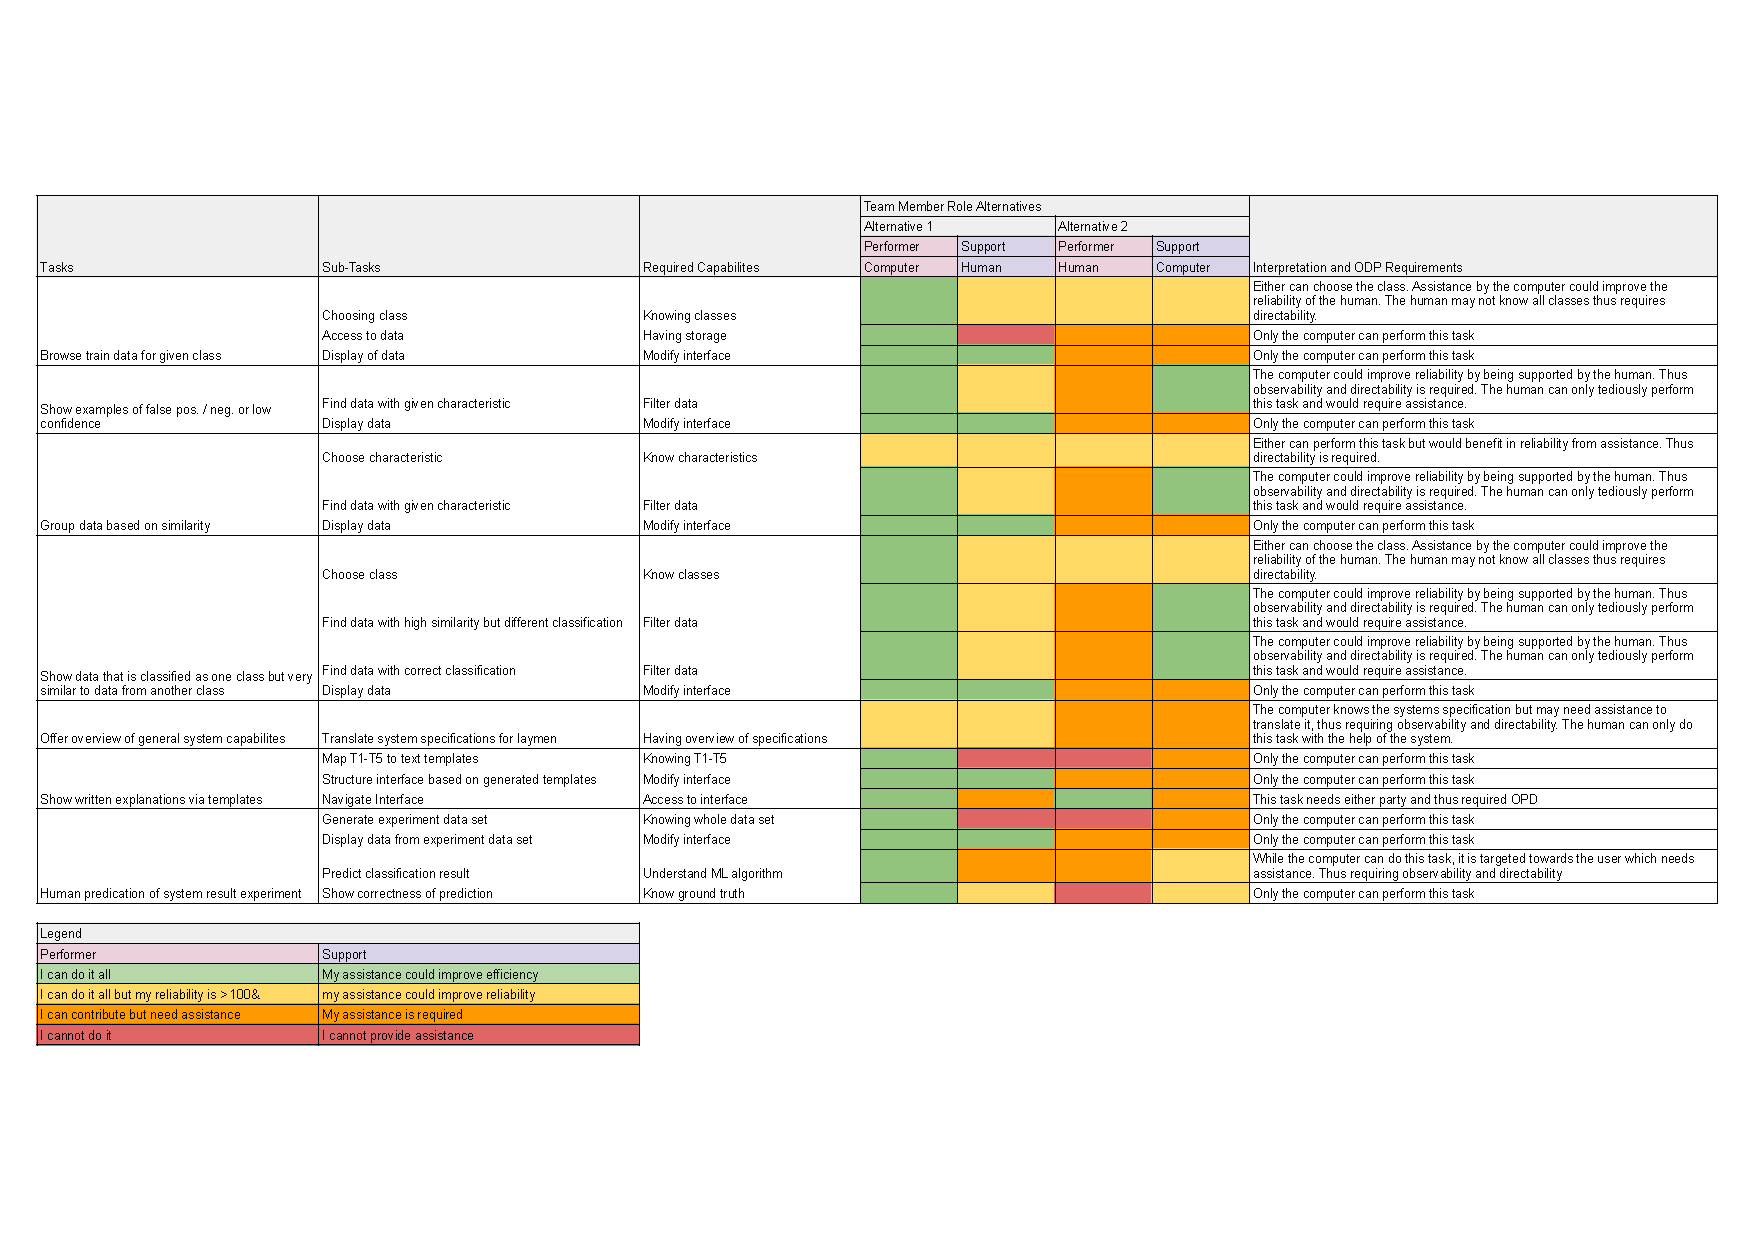
\includegraphics[height=\textwidth, angle=90]{img/figures/Interdependency_Analysis_Table.pdf}
    \caption{Interdependency Analysis Table}
    \label{table:interdependency_analysis_table}
\end{table}

\subsection{Explanation Techniques}\label{subsection:explanation_techniques}
Three groups of explanation techniques are created as possible ways to implement the required functionalities (\autoref{table:function_specification}). The groups are divided by their style of interaction and information deliverance. Most of the presented techniques have a direct mapping to the functionalities to be provided by the assessment system, especially \textit{General Description, Metrics, Data Browsing and Experiment}. The visual explanation techniques though, do overlap significantly in their practicality. While they differ drastically in their mode of operation and technical background, they do cater to the same interaction: Showing image regions that are significant to the result of the AI. Because of this and the limited time and resource frame, only one of the three proposed visual explanation types will be implemented.
\subsubsection*{Textual}
\begin{description}[font=\normalfont\itshape]
    \item[General Description:] General descriptions of the system capabilities aim to explain the system on a level, that is accessible to machine learning laymen, such as medical professionals. As described by \textcite{people_ai_google_website} it is beneficial for building trust when the system capabilities are explained instead of the technology itself. This helps the user to build a better mental model, especially when dealing with hyper-complex structures, such as DNNs. The general descriptions shall contain a textual explanations of the model capabilities to ensure a good introduction and appropriate expectations.
    \item[Metrics:] Standard metrics are also used to describe the machine learning model. The metrics used are \textit{Accuracy, Precision, Recall \& F1}. Those metrics were chosen, because they are often used to describe other processes and applications in the medical context and therefore should be familiar and interpretable by the user. 
\end{description}

\subsubsection*{Interactive}
\begin{description}[font=\normalfont\itshape]
    \item[Data Browsing:] The ability to browse the training data of a machine learning model was universally requested by the interviewed professionals. The browsing ability is extended by different filters for the specific functionality. The user shall be able to explore the training data based on the class of the image. Furthermore the data will be algorithmically grouped based on similarities to potentially expose patterns. Additionally the user shall be able to explore data points that belong to the edge cases of the models capabilities, such as false negative and false positives.
    \item[Experiment:] Comparing the machine learning models predictions to the human expertise also was a key aspect of AI interaction in the medical domain as shown by the interviews. Therefore a input-output-experiment shall be implemented, where the user is able to test the AI against its own expertise.
\end{description}

\subsubsection*{Visual}
\begin{description}[font=\normalfont\itshape]
    \item[Occlusion:] A perturbation based approach to compute attribution, involving replacing each contiguous rectangular region with a given baseline, and computing the difference in output. Occlusion is most useful in cases such as images, where pixels in a contiguous rectangular region are likely to be highly correlated \parencite{captum_website,zeiler_visualizing_2013}.
    \item[Anchors:] The algorithm provides model-agnostic and human interpretable explanations suitable for classification models applied to images, text and tabular data. The idea behind anchors is to explain the behaviour of complex models with high-precision rules called anchors. These anchors are locally sufficient conditions to ensure a certain prediction with a high degree of confidence \parencite{ribeiro_anchors_2018}.
    \item[LRP:] The Layer-wise Relevance Propagation (LRP) algorithm explains a classifier's prediction specific to a given data point by attributing (positive \& negative) relevance scores to important components of the input by using the topology of the learned model itself \parencite{lapuschkin_unmasking_2019}.
\end{description}
Referencing the \autoref{chapter:analysis}, the main goal of a visual explanation shall be the validation of the AI model's behavior. Therefore a simple technique, such as Occlusion, which only highlights image regions with a high importance to a result, is reasonable to implement. While LRP does have certain benefits because of its ability to assess positive and negative influences of pixels to the model output, it also comes with a high complexity that manifests as a lot of hyperparameters, making it hard to implement and use properly. Anchors work differently to the other two methods, since it is able to find a hyperpixel that is most influential to a AI's classification. In the context of standardized medical images, that are already preprocessed in a certain way (e.g. X-ray images), the method looses it's edge. The high similarity of images in medical binary classification tasks lessens the expressiveness of Anchors significantly.    

\section{System Architecture}\label{section:system_architecture}
The goal is to create an interactive software application, therefore a suitable system architecture has to be constructed to suite the needs of the users and the usage context. Although, implementing the functionalities from \autoref{section:functionalities} is possible in many different ways. It is possible to realize the assessment system as a classical, offline software application or by leveraging web based tool sets for a possibly distributed cloud solution. Also it is conceivable to implement the system on a middle ground of those two, by creating a software that is build to be ran locally in common web browsers. To stay hardware and software agnostic these three options will be shortly evaluated against each other based on the requirements set by the functionalities.

The common requirements are the ability to store machine learning models and training data for the assessment to be computed. In addition the user has to be presented with a graphical user interface (\textbf{GUI}) to interact with. Having these two components in a close relation can drastically reduce the overhead of implementing the communication between the computational and data storage component with the GUI component. On the other hand such a close relation in an offline system can significantly reduce the flexibility of the implementation regarding GUI and interaction design. Furthermore a single offline application has to take many different execution environments (operating systems) into account, which might be a big downside depending on the actual context of usage. Separating the system into a multi-tier application allows for more modularity and freedom in choosing the actual implementation technology. A multi-tier web application allows for a very specialized choice of tools for the respective component at the cost of a higher complexity and implementation cost. Such web applications have the advantage of being relatively easy to transform into a local application without the need of hosting a server environment. This can be the middle ground between the offline local and the web based distributed application.

Referencing the usage context of the application it is not needed to implement a highly complex distributed application, although Clearbox has shown that it is very much possible to implement a robust cloud based solution. To reduce the scope of implementation for this thesis a middle ground is the most reasonable: Leveraging modern web based tools that are mostly environment agnostic to build a flexible application that could be ran in either the cloud or locally on a single machine.

\section{Interaction Design}\label{section:interaction_design}
The interaction design is a key aspect of human-computer-interaction, as it defines how the user will actually interact with the system and how information will be made accessible to the user. Considering the human factors in the design process is very important as described by \textcite{wickens_2016_engineering} - for this builds upon the insights of the previous chapters, namely the definition of interaction (sub-)tasks and the interdependency analysis, which in turn are based on the general objectives and user needs as described in \autoref{chapter:analysis}.

The conception of functionalities and interaction design was the main topic of the previously mentioned expert workshop, which was conducted with colleagues from the University of Lübeck and Clearbox. The goal was to present, validate and discuss the scope of functionalities (based on the previous research and the user requirements) and the interaction design which utilizes scaffolding and guidance for the main user group. The workshop yielded good feedback on the scope of functionalities and the guidance idea. A main focus of the discussion was type of guidance which was then resolved to a semantic signal manifested by an intention query.

A central consideration of the interaction design is to adapt the system to the abilities and needs of the actual users. Referencing \autoref{subsection:interviews}, a main user group has low expertise in machine learning, which in turn means special requirements for the interaction design of an AI assessment system. Therefore the design approach will revolve around a guided interaction version and a unguided interaction version: The guided interaction will leverage a more streamlined approach which facilitates the intentions of the user by asking and then presenting the respective functionality. \textcite{trigg_guided_1988} already proposes local guidance of the user by the author of a system, by using intention queries to determine a suitable path through the content of an application. This mode of interaction aims to relieve the user of mental workload by scaffolding the application and thus avoiding the presentation of all functionalities, and therefore aiding the learning process for machine learning topics \parencite{soloway_learner_1994}. The other mode of interaction will be unguided, as in there will be no intention query and the user will be able to freely explore the whole lot of functionalities offered by the application, which is hypothesize to be beneficial for users with more expertise in machine learning. The baseline for both ways of interaction is the whole array of functionalities as specified in \autoref{table:function_specification}.

To further explore and concretize the interaction design two methods were applied: \textit{Interaction Dialogues} and \textit{Interaction Flowcharts}. Interaction dialogues aim to creatively explore different ways of implementing the functionalities as defined in \autoref{section:functionalities}. Additionally they enable the exploration of other perspectives based on a natural interaction mode (spoken dialogue). The result is then the baseline for the interaction flowcharts, which specify the concrete flow of information in a standardized manner.

\subsection{Interaction Dialogues}\label{subsection:interaction_dialogues}
The idea of using interaction dialogues to creatively explore different ways of interacting with the assessment system came from the cooperation with Clearbox. A colleague specialized in building User Interaction and User Experience proposed this method to be used for developing the interaction design. Using dialogues as the mode of interaction and communication between human and computer allows for a very liberated design process. The goal was to explore different variations of interaction based on the functionalities as defined in \autoref{table:function_specification}. An example dialogue (with H for human and C for computer) for task 1 will be presented:
\begin{displayquote}
    H: I would like to see your training data.\\
    C: Do you want to see all data or just data for a specific class?\\
    H: I want to only see data for class x.\\
    C: Here you go! Do you want to see data of another class, too?\\
    H: Yes please, but give me some time.\\
    C: Of course!
\end{displayquote}

Using the dialogue technique allows for easy exploration of alternative information flows as shown by the next example:
\begin{displayquote}
    H: I would like to see your training data.\\
    C: Here take a look!\\
    H: Wow, that is really a lot!\\
    C: Do you want to filter for a specific class?\\
    H: Yes, please show me only data for class x.\\
    C: There you go.\\
    H: Thank you, and now please show me all data for class y.\\
    C: Sure, here!
\end{displayquote}

These examples clearly show different ways of interacting in order to accomplish the same task: Browsing the training data. This process was applied to all tasks (and sub-tasks) from \autoref{table:interdependency_analysis_table} to gather a lot of different interaction variations, to be then used as a baseline for the following interaction flowcharts. The key takeaways from this process, was that there are various possibilities to realize an interaction. With multiple alternatives per task, some comparisons could be made: Often it seems beneficial for a streamlined interaction design, to present the user with a set of options from the beginning, instead of presenting everything and then reducing the amount of information. Furthermore situations with exhaustive searches can be avoided by presenting the user a limited amount of information. Most tasks had two to three alternatives which were compared against each other in order to find the best dialogue, which was then chosen to be the baseline for the standardized flowcharts.

\subsection{Interaction Flowcharts}\label{subsection:interaction_flowcharts}
Building on the previous chapters the possible human-computer-interactions were formalized into flowcharts. The type of flowchart is defined in \textit{DIN 66001} \parencite{hering_programmablaufplan_1984}. The flowcharts are essential as a reference for the implementation, as they define the details of the information flow between the two parties. The goal is to have interactions that have a clear start and end point, with no dead ends - leveraging flowcharts for this allows for an easy validation of these goals. Another goal was to separate the application into smaller, more manageable pieces, each defined by its own flowchart. \autoref{fig:flowchart_browse_data} shows a flowchart that defines the flow of interaction for the process of browsing classified images (task 1 from \autoref{table:function_specification}), with the background of the presented interaction dialogue. For each of the tasks defined in \autoref{table:function_specification} and \autoref{table:interdependency_analysis_table} such a flowchart was developed as seen in \nameref{appendix:interaction_flowcharts}.
\begin{figure}[htbp]
    \centering
    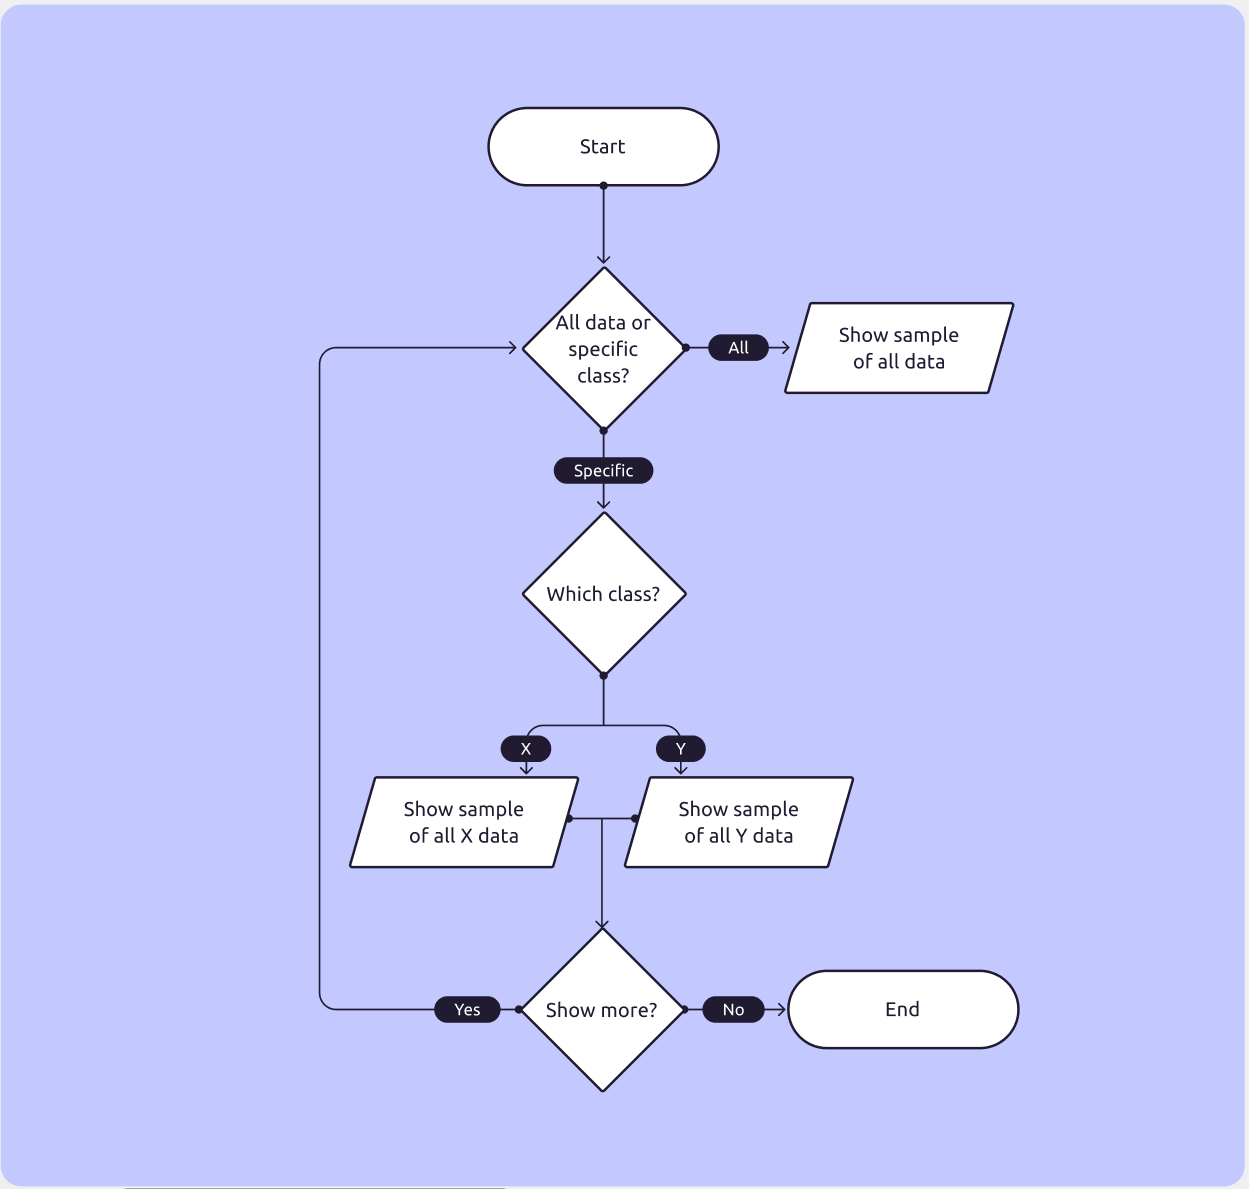
\includegraphics[width=\textwidth]{img/figures/flowcharts/browse_train_data_for_chosen_class.png}
    \caption{Flowchart - Browse Training Data for a given Class}
    \label{fig:flowchart_browse_data}
\end{figure}

\section{Interface Design}\label{section:interface_design}
Building on the functional specification and the interaction design an interface design was developed to encompass the whole array of functionality into a single application. Similar to the flowcharts the application interface will be split up into single elements of interaction as defined by the tasks and interaction flowcharts. This separation allows for a better overview and a more flexible layout. Additionally inspiration was drawn from the state-of-the-art application from Clearbox as seen in \autoref{section:state_of_the_art}, where a similar approach was chosen. The concept of splitting the application into smaller pieces also facilitates the usability of the whole application, as the user will not be overburdened with all functionalities simultaneously. Instead the user will be able to choose which functionality he wants to utilize. This layout goes hand in hand with the guidance concept, as every functionality will be represented by its own part of the user interface. This is an important aspect to consider, especially regarding the reusability of software components. Furthermore, preventing multiple implementations of the same functionality helps with the comparability of the guided versus non-guided version of the application.

The application is conceived for devices with relatively big screen sizes, such as desktop computers, laptops or tablets as there was no use case found for a mobile application (see \autoref{chapter:analysis}). Additionally the screen size is needed for the user to properly view the image content. As such the layout of the application will be vertically scrollable, optimized for landscape orientations to match the devices and the use case.

\autoref{fig:mockup_part_1}, \autoref{fig:mockup_part_2} and \autoref{fig:mockup_part_3} show a mockup of the application, designed as a single page layout with all functionalities present. The layout presented here corresponds to the unguided version. On the top of the application (\autoref{fig:mockup_part_1}) general information about the model, its capabilities and standard metrics are shown. Further down (\autoref{fig:mockup_part_2}) the data browsing functionalities are depicted. Lastly the the similarities and the experiment functionalities are shown at the bottom of the application (\autoref{fig:mockup_part_3}). Furthermore the order of the components is determined by the level of involvement needed of the user: The beginning is limited to higher level information, which then transforms into a deeper insight into the training data, model limitations and clustering of data, and concludes in the input-output experiment where the user can test its mental model against the actual AI.

The general design of the application revolves around a simple modern layered design in the form of cards with rounded corners. This aims to make the single components easily distinguishable while preventing the introduction of unnecessary visual separations. The color theme of the application is chosen to be neutral with high contrast between text and background while utilizing highlighting colors for important interface components for good readability and easy orientation. Although this mockup heavily references Clearbox' design language, a additional dark mode with inverted colors is considered depending on the user preferences and image content.

\begin{figure}[htbp]
    \centering
    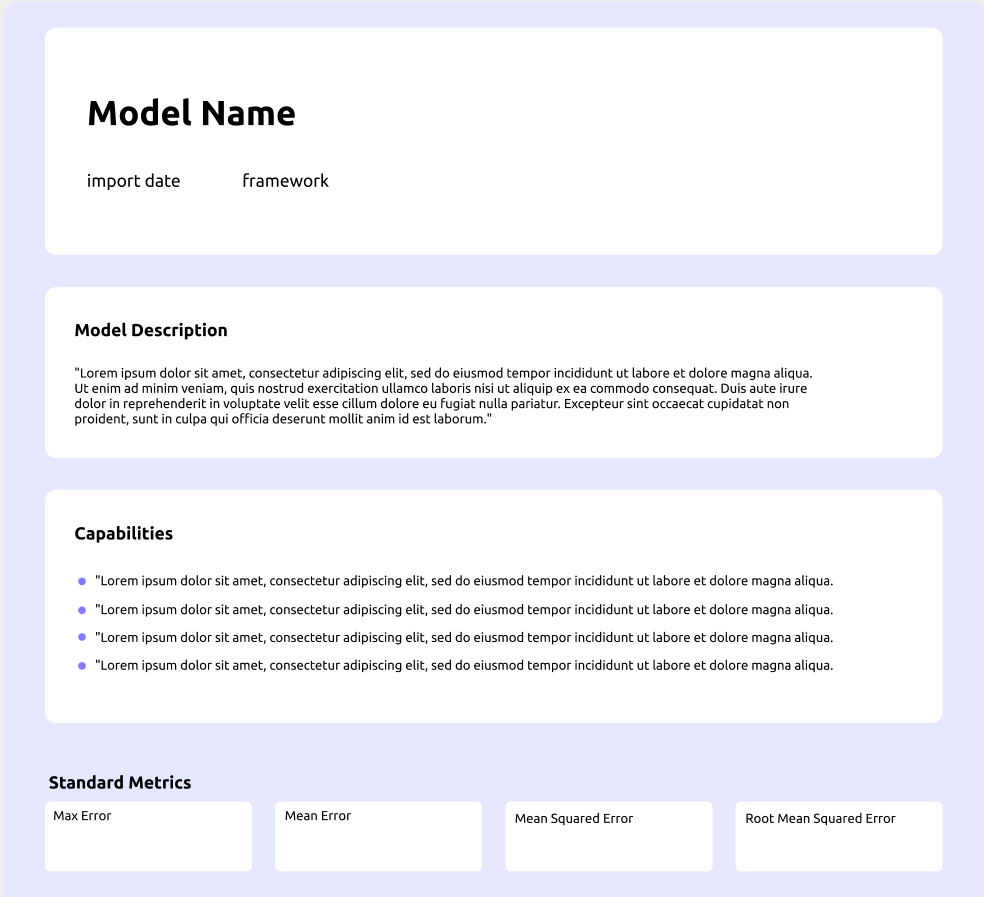
\includegraphics[width=\textwidth]{img/figures/mockups/mockup_1.png}
    \caption{Mockup Part 1}
    \label{fig:mockup_part_1}
\end{figure}

\begin{figure}[htbp]
    \centering
    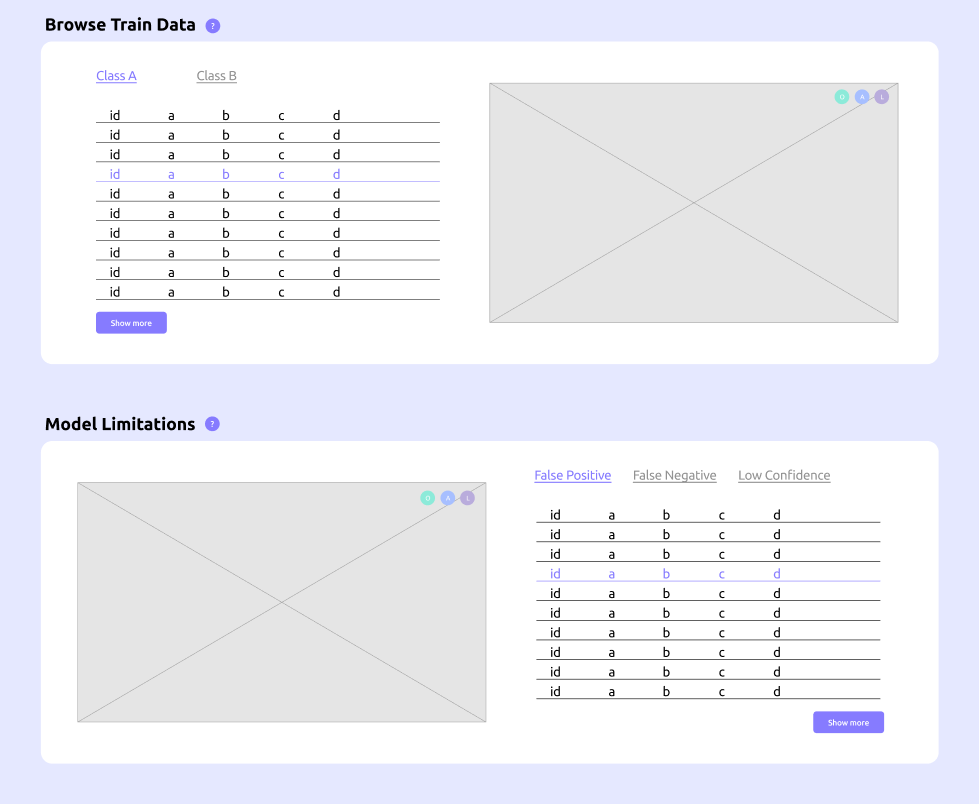
\includegraphics[width=\textwidth]{img/figures/mockups/mockup_2.png}
    \caption{Mockup Part 2}
    \label{fig:mockup_part_2}
\end{figure}

\begin{figure}[htbp]
    \centering
    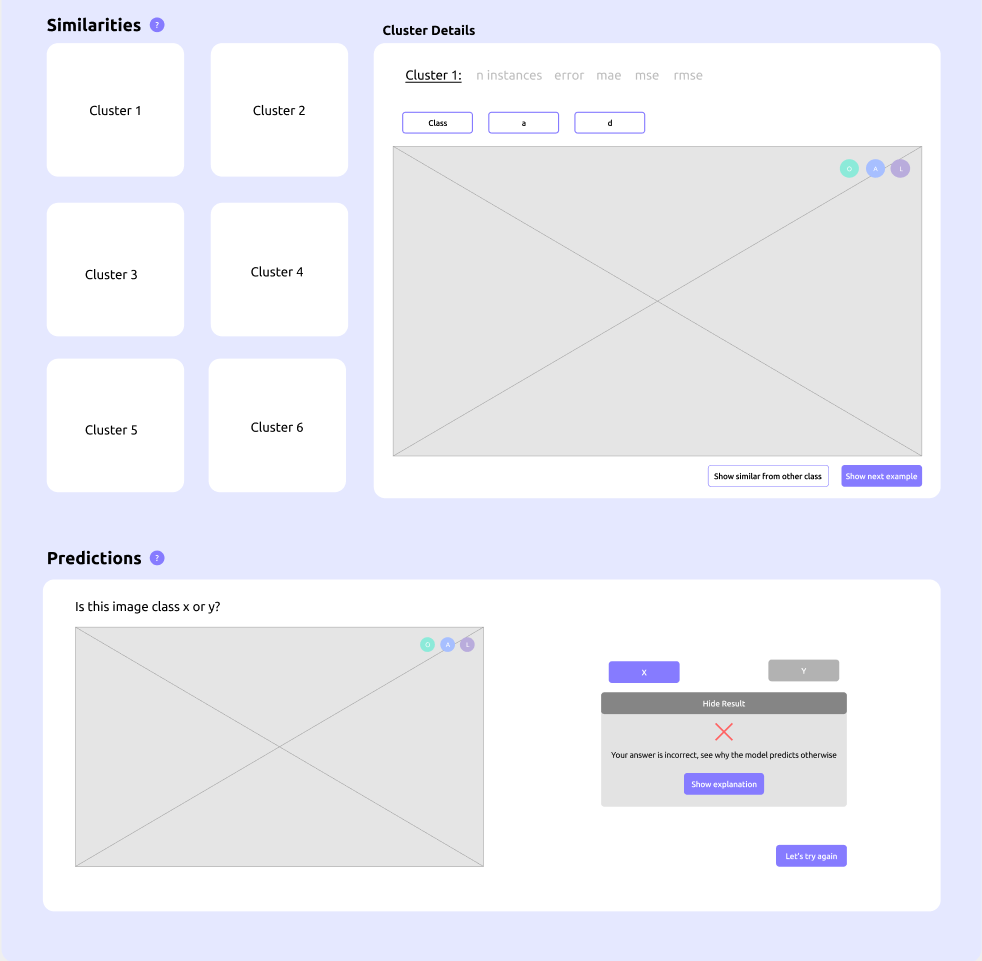
\includegraphics[width=\textwidth]{img/figures/mockups/mockup_3.png}
    \caption{Mockup Part 3}
    \label{fig:mockup_part_3}
\end{figure}

\section{Conclusion on the Conception}
Building on the analysis, the conception conceived possible solutions to meet the requirements of the user, the usage context and the overall goals. By referencing the concrete use cases and user requirements seven functionalities were derieved (\autoref{table:function_specification}), which were then analysed for interdependencies in a human-computer-interaction scenario (\autoref{table:interdependency_analysis_table}), resulting in a clear specification of tasks, sub tasks and capabilities required to perform those for either party of the interaction. Furthermore The functionalities were described in detail in \autoref{subsection:explanation_techniques} and insights were collected about the mapping of the functionalities to the explanation techniques, while providing a semantic grouping for those techniques. Although many explanations techniques have a direct mapping, the visual explanation was overrepresented and therefore one from three options was chosen. Having the functional specification set, allowed for the development of a system architecture (\autoref{section:interface_design}), which is constructed with flexibility in mind and leveraging modern web based technologies while still meeting the requirements of an AI assessment system. Through a conceptional iteration via an expert workshop the ideas were further discussed and deepened, resulting in interaction dialogues (\autoref{subsection:interaction_dialogues}) for the seven tasks and subsequently in interaction flowcharts (\autoref{subsection:interaction_flowcharts}) defining the concrete flow of information between the interacting parties. Finally those functional components were manifested in an interface design (\autoref{section:interface_design}), which leverages the interaction design and the idea of guided versus non guided interaction styles to provide a easy to understand GUI for users with low expertise in machine learning. While taking clear reference to Clearbox's design concept and language, the concept here aims to provide two different GUIs that build on the same flexible components, each encompassing one functionality, to be later evaluated against each other.

\newpage
\chapter{Implementation}\label{chapter:implementation}
The AI assessment system will be implemented based on the insights and ideas from \autoref{chapter:conception}. Although the system to be build has to realise many tasks from the data science and machine learning domains, it also needs to provide a GUI for user interaction, as described by \autoref{section:system_architecture}. Taking these aspects into account, a \textit{Python} based implementation is preferable, as the programming language is widely used for data science and machine learning tasks, while also providing tools for GUI and web application building. Furthermore Python ranks the most popular programming language, while providing some of the most used and curated software libraries for data science and machine learning among all alternatives \parencite{toibe_index_python_website,numpy_github,pandas_github,pytorch_website}.

Referencing \autoref{subsection:existing_apps} and Clearbox, a Python based application leveraging \textit{Streamlit} will be used for implementing the AI assessment system \parencite{streamlit_website}. While there are many different possible alternatives to implement such a flexible distributed system (for example \textit{Django} or \textit{Flask}), Streamlit comes with a big advantage: The ability to directly transform Python scripts into deployment ready web applications including a GUI. This ability completely invalidates the disadvantage of building a flexible web based application, as it avoids the additional effort of implementing the communication between the presentational and the logic layer of a multi-tier application. Although strictly speaking a Streamlit-based application will not be multi-tiered in its implementation as it only consists of singular python scripts leveraging the Streamlit platform, which in turn hides most of the complexity of implementing a distributed, web based implementation. Additionally some flexibility in implementing the actual front end of the application is lost by using such a omnipotent library, as there is no need for a specialized front end technology. However it is reasonable to limit the implementation of a AI assessment system prototype in the scope of this thesis.

\section{System Architecture Implementation}
\begin{comment}
vgl. Konzeption, jetzt aber wie und womit es konkret umgesetzt wurde (u.U. bieten sich UML-Diagramme an)
\end{comment}

Text \dots

\section{Interface Implementation}
\begin{comment}
vgl. Konzeption, jetzt aber wie und womit es konkret umgesetzt wurde 
\end{comment}

Text \dots

\section{Conclusion on the Implementation}
\begin{comment}
Kurzes Fazit, das u.a. die Frage beantwortet, was technisch konkret umgesetzt wurde und was z. B. aus der Konzeption übrig geblieben ist und warum.
\end{comment}

Text \dots

\newpage
\chapter{Dialogue Samples}
\begin{comment}
Verdeutlichen Sie die Funktionsweise Ihre Entwicklung bei einer typischen Bedienung (z. B. wie in einem Anwendungsbeispiel / Use Case beschrieben — auf den können Sie sich ja beziehen).

Die Abbildungen müssen im Text vorher erläutert sein und einen Eindruck geben, wie die Entwicklung konkret bedient wird bzw. was sie kann.

\textbf{Das ist das, was bleibt:} Diese Dialogbeispiele sind das einzige, was in ein paar Jahren von Ihrer Anwendung noch sichtbar ist. Dann ist entweder der Datenträger verschwunden oder beschädigt oder die notwendige Hard- und Software ist nicht mehr lauffähig. Geben Sie dem Leser entsprechend einen guten Einblick in das, was Sie tatsächlich realisiert haben.

\textbf{Jetzt ein Video aufnehmen:} Schalten Sie den Screenrecorder auf dem Computer (not-falls: QuickTime) oder Smartphone (kann das OS) an und nehmen Sie die typischen Interaktionen einmal auf. Das ist Ihr "Plan B", falls (oft: wenn) im Kolloquium die App nicht bedient werden kann. Das können Sie auch gut auf DVD brennen um Lesern die Möglichkeit geben, sich die Interaktion anzusehen (in der Arbeit darauf hinweisen!). Macht sich auch gut auf Websites (insbesondere dem eigenen Portfolio).
\end{comment}

Text \dots

\newpage
\chapter{Summative Evaluation}\label{chapter:evaluation}
\begin{comment}
Geben Sie zu Beginn der Evaluation einen kurzen Überblick über Ihr Vorgehen. Dazu reichen meist die Zwischenüberschriften mit ein oder zwei Sätzen, was Sie konkret gemacht haben. Also nicht "In Design wird das Design beschrieben" sondern "Das experimentelle Vorgehen wird im Abschnitt Design dargestellt".
\end{comment}

Text \dots

\section{Goal}
\begin{comment}
Die summative Evaluation ist eine abschließende Bewertung Ihrer Entwicklung. Ziel ist, unter dem Strich zu sehen, wie gebrauchstauglich Ihr System ist (nicht mehr eine iterative Verbesserung wie in der formativen Evaluation der Konzeption). Da-für müssen Sie klare Kriterien ableiten, was eine "gute" bzw. "schlechte" Bewertung nach sich ziehen würde. Meist sind das die klassischen Gebrauchstauglichkeitskriterien (Effektivität, Effizienz, Erlernbarkeit, Zufriedenstellung), wobei diese über das Ziel Ihrer Anwendung konkretisiert werden (Effektivität bei einer Lernapp ist konkret gemessen etwas anderes als Effektivität bei einem digitalen Depressionstagebuch).

Hier verdeutlichen Sie entsprechend, welche Fragen die Evaluation beantworten soll.
\end{comment}

Text \dots

\section{Methods}
\begin{comment}
Im Methodenteil zeigen Sie, was wie evaluiert wurde. Der Methodenteil muss anderen Entwicklern die Möglichkeit geben, Ihr Evaluationsvorgehen zu wiederholen um Ihre Ergebnisse zu überprüfen. 
\end{comment}

Text \dots

\subsection{Design}
\begin{comment}
Kurze Beschreibung des Versuchs- oder Evaluationsdesigns, dass man das Vorgehen einordnen kann. Also z. B. "es wurde ein Usability Test durchgeführt", oder "es wurde ein Experiment mit between-subjects design durchgeführt, bei dem die Kontrollgruppe die bisherige App verwendet hat und die Experimentalgruppe die neu entwickelte App".
\end{comment}

Text \dots

\subsection{Participants}
\begin{comment}
Kurze Beschreibung der Teilnehmer mit relevanten Angaben. In jedem Fall die Anzahl, oft noch Geschlecht, Alter, Beruf, Vorerfahrung, etc. Bei weniger als zehn Teilnehmern bietet sich eine Tabelle zur schnellen Übersicht an. Verweisen Sie bei individuellen Ergebnissen (z.B. Zitaten aus Fragebögen oder Interviews) auf die Teilnehmer-Nummer.

Achtung: Niemals die Namen der Teilnehmer erwähnen! Die Teilnehmer stehen stellvertretend für die Zielgruppe. Wer sie konkret sind ist irrelevant. Begründen Sie, warum Sie diese Personen ausgewählt haben (spiegeln die Nutzergruppe gut wider) und wo/wie Sie diese rekrutiert haben.
\end{comment}

Text \dots

\subsection{Setting and Instruments}
\begin{comment}
Beschreiben Sie die notwendigen Materialien bei der Evaluation. Dazu gehört — mit Überschriften klar ausgewiesen — das Setting (wo wurde die Evaluation durchgeführt), Ihre Entwicklung (Verweis auf Dialogbeispiele), und Ihre Erhebungsmethoden (Fragebögen, Interviewleitfäden, etc.).

Falls Sie etablierte Fragebögen verwenden (z.B. ATI) reicht die entsprechende Zitation mit einer kurzen Beschreibung. Bei längeren Fragebögen oder Interviewleitfäden nennen Sie kurz die Abschnitte (z.B. soziodemographische Daten, Technikerfahrung, etc.) und verweisen Sie auf die vollständigen Fragebögen im Anhang.

\textbf{ACHTUNG:} Zeitliche Reihenfolge ist hier egal. Hier geht es nach Gliederungspunkten wie Instrumente (Fragebögen, Interviews, etc.). Die zeitliche Reihenfolge wird in der Prozedur dargestellt.
\end{comment}

\paragraph{Setting}\mbox{} \\
Text \dots

\paragraph{Verwendete Anwendung}\mbox{} \\
Text \dots

\paragraph{Fragebögen}\mbox{} \\
Text \dots

\subsection{Procedure}
\begin{comment}
Beschreiben Sie chronologisch den Ablauf der Evaluation, von der Begrüßung bis zur Verabschiedung. Verweisen Sie dabei auf die anderen Abschnitte (v.a. Setting und Instrumente) und führen Sie nichts Neues mehr ein. Dieser Abschnitt ist der einzige Abschnitt, in dem Sie die zeitliche Reihenfolge klar einhalten müssen, alle anderen sind inhaltlich strukturiert.
\end{comment}

Text \dots

\begin{comment}
Nach dem Lesen der Methode muss deutlich geworden sein, wie Sie Ihre Evaluationsfragen messbar gemacht haben. Wie haben Sie z.B. Benutzerzufriedenheit oder Effizienz gemessen? Die Leser müssen sich aufgrund des Methodenteils in die Lage der Teilnehmer versetzen können und ein mentales Modell Ihrer Evaluation bilden können.
\end{comment}

\section{Results}
\begin{comment}
In den Ergebnissen zeigen Sie wie die Ergebnisse analysiert wurden um Ihre Evaluationsfragen zu beantworten. Nicht einfach die Daten auflisten, sondern stellen Sie die Ergebnisse strukturiert dar und betonen Sie die wichtigen Aspekte. Gliedern Sie die Ergebnisse nach Ihren Forschungsfragen / Fragestellungen (nicht zeitlich oder nach Erhebungsmethoden wie Fragebögen vs. Beobachtung). Zu Beginn (falls relevant) sollten Sie überprüfen, ob die Anwendung auch wirklich so verwendet wurde, wie sie verwendet werden sollte (manipulation check). Haben die Personen also z. B. wirklich die Aufgaben mit der App gelöst oder haben sie die App schnell beiseite gelegt.

Stellen Sie die Befunde / Ergebnisse von Analysen / Evaluationen / etc. immer so neutral und so objektiv wie möglich dar — ohne Ihre subjektive Interpretation oder Bewertung. Also keine Begriffe wie "lediglich", "nur", "könnte / würde / sollte / etc." oder Bewertungen wie "hat gut / nicht gut geklappt". Diese Bewertungen gehört in die Diskussion.

Überlegen Sie sich mit welchen Tabellen und Abbildungen Sie die Ergebnisse gut darstellen können. Bei aggregierten Messwerten (auf mindestens Intervallskalenniveau) immer Mittelwerte (M), Standardabweichungen (SD) und die Anzahl der Messdaten (Personen, n) angeben. Bei ordinalskalierten Daten entsprechend Median, etc. (ja, Statistik war wichtig).

Statistische Tests korrekt angeben (siehe z.B. Pallant, 2010).

Pallant, J. (2007). SPSS Survival Manual (3rd ed.). Open University Press.

Abbildungen müssen in sich verständlich sein (was abgebildet ist). Das heißt, die Achsen eindeutig beschriften, Skala (z.B. Likert-Skala von 1 starke Ablehnung bis 7 starke Zustimmung) in die Legende. 3D-Graphiken vermeiden — diese bieten oft keinen Mehrwert (vgl. Field, 2016).

Field, A. (2016). An Adventure in Statistics. Sage.

Am Ende des Ergebnis-Abschnitts muss deutlich geworden sein, wie Ihre Entwicklung von den Teilnehmenden eingesetzt wurde (hoffentlich wie geplant), was die Hauptergebnisse waren, sofern aufgrund der Stichprobengröße möglich welche Werte sich statistisch signifikant voneinander unterscheiden und was die statistischen Ergebnisse in den Variablen bedeuten (z. B. positive Korrelation zwischen A und B, dass Personen, die A besser bewertet haben auch B besser bewertet haben; aber keine Bewertung ob das gut oder schlecht ist). Falls Sie konkrete Ziele hatten (z. B. "SUS-Wert von x") dann sagen Sie, ob dieses Ziel erreicht wurde oder nicht (das ist keine Wertung, die in die Diskussion gehören würde, sondern ein größer, gleich oder kleiner was eindeutig ist).
\end{comment}

Text \dots

\section{Discussion}
\begin{comment}
In der Diskussion erklären und interpretieren Sie die Ergebnisse. Welche Schlussfolgerungen ziehen Sie daraus? Was sind die praktischen Konsequenzen für die (weitere) Entwicklung? Hier dürfen Sie selbst die Ergebnisse bewerten — auf Basis von einer kritischen Reflektion.
In der Diskussion keine neuen Ergebnisse aus der Analyse / Evaluation / etc. einführen. Die Beweisaufnahme ist mit Ende des Ergebnisteils abgeschlossen. Es geht hier auch nicht um eine Mystery-Geschichte mit Spannungsbogen, sondern um klar nachvollziehbare Argumente. Neue Informationen aus der Literatur verwenden um die (v.a. überraschende) Ergebnisse zu interpretieren ist dagegen möglich.
\end{comment}

Text \dots

\section{Conclusion on the Evaluation}
\begin{comment}
Fassen Sie die Evaluation kurz zusammen — insbesondere was die zentralen Ergebnisse waren. Unterm Strich: Wie gut hat's geklappt?
\end{comment}

Text \dots

\newpage
\chapter{Summary and Outlook}
\begin{comment}
Kurze Einführung, was in den folgenden Unterkapiteln behandelt wird.
\end{comment}

Text \dots

\section{Summary}
\begin{comment}
Fassen Sie die zentralen Schritte und Ergebnisse Ihrer Arbeit kurz zusammen. Personen mit wenig Zeit müssen aus dieser Darstellung die Kernpunkte Ihrer Arbeit mit-nehmen und Ihren Arbeitsaufwand und Erfolg bewerten können.

Ist ähnlich wie die Zusammenfassung zu Beginn der Arbeit, aber etwas länger (1 bis maximal 2 Seiten) mit Verweisen auf die entsprechenden Kapitel/Abschnitte und Sie können beim Leser etwas mehr voraussetzen (hat es gelesen oder kann wegen den Verweisen direkt dahin springen).
\end{comment}

Text \dots

\section{Outstanding Issues}
\begin{comment}
\textbf{Offene Punkte = Versprochene aber nicht umgesetzte Punkte:} Falls Schritte explizit geplant wurden (Exposé! Pflichtenheft!), aber nicht realisiert werden konnten, dann diese hier klar darstellen und diskutieren.

Mögliche Features, die Sie nicht vor Beginn versprochen haben, gehören in den Ausblick.
\end{comment}

Text \dots

\section{Outlook}
\begin{comment}
Ideen, welche weiteren Entwicklungen oder Untersuchungen folgen sollten, oder was man noch umsetzen könnte, gehören in den Ausblick.

Versprochene aber nicht umgesetzte Elemente in die Offenen Punkte.

Bitte keine Allgemeinheiten ("können noch Features hinzugefügt werden" oder "könnte besser evaluiert werden") sondern konkrete Beschreibungen und Begründungen der Relevanz dieser Schritte.
\end{comment}

Text \dots

\section{Final Conclusion}
\begin{comment}
Die Arbeit, die Ergebnisse und weitere mögliche Schritte kurz kritisch (ehrlich und konstruktiv, aber nicht selbstkreuzigend) reflektieren und positiv enden. Maximal eine halbe bis 3/4 Seite.
Ist kurz und hier können Sie von der Arbeit zurücktreten und auch den Leser aus dem Text ziehen.

Das ist nur zum Test: \textcite{ford} \textcite{hadoop}
\end{comment}

Text \dots

\clearpage
\phantomsection
\addcontentsline{toc}{chapter}{Abbildungsverzeichnis}
\listoffigures
\clearpage

\phantomsection
\addcontentsline{toc}{chapter}{Tabellenverzeichnis}
\listoftables
\clearpage

\phantomsection
\addcontentsline{toc}{chapter}{Quellen}
\chapter*{Quellen}

\phantomsection
\printbibliography[heading=subbibintoc, nottype=online, nottype=software]

\phantomsection
\printbibliography[heading=subbibintoc, type=online, title=Websites]
\begin{comment}
Websites haben nicht die gleiche Fundierung/Überzeugungskraft wie wissenschaftliche Literatur (peer-review/Anspruch). Die Websites separat aufzuführen, macht es einfacher zu sehen, was wirklich wissenschaftlich fundierte Literatur ist.
\end{comment}

\phantomsection
\printbibliography[heading=subbibintoc, type=software, title=Software]
\begin{comment}
Software-Name mit Versionsnummer und Link zur Website. Nur was für die konkrete Arbeit relevant ist. Das Sie die Arbeit mit Word geschrieben haben, ist irrelevant. Das sieht man. LaTeX auch.
\end{comment}
\clearpage

\phantomsection
\addcontentsline{toc}{chapter}{Abkürzungen}
\chapter*{Abkürzungen}
\begin{comment}
Kann recht kurz ausfallen, aber falls Sie bestimmte Abkürzungen häufiger verwenden, hier aufführen. Geht nur darum, dass der Leser hierhin blättern könnte, wenn er über eine unbekannte Abkürzung stolpert. Ist beim digitalen Lesen hinfällig geworden. Hier geht es wirklich nur um Akronyme, z. B. ICBM = Intercontinental Ballistic Missile, oder PIN = Personal Identification Number. Die Erläuterung von Begriffen erfolgt im Glossar.
\end{comment}

\begin{description}
    \item [\textbf{Akronym}] Ausgeschriebenes Akronym
\end{description}
\clearpage

\phantomsection
\addcontentsline{toc}{chapter}{Glossar}
\chapter*{Glossar}
\begin{comment}
Unterschiedliche Disziplinen verwenden z. T. die selben Begriffe für unterschiedliche Sachverhalte und unterschiedliche Begriffe für die selben Sachverhalte. Hier können Sie wiederkehrende zentrale Begriffe der Arbeit kurz definieren (z. B. Adipositas, Depression, Legasthenie, etc.). Früher wichtiger, dann konnte man hierhin blättern und musste nicht den ganzen Text absuchen. Heute verwendet man digital die Suchfunktion. Trotzdem ernst nehmen.
\end{comment}

\begin{description}
    \item [\textbf{Begriff}] Kurze Erläuterung
\end{description}
\clearpage

\phantomsection
\addcontentsline{toc}{chapter}{Anhänge}
\chapter*{Anhänge}
\begin{comment}
Zusätzliche Informationen die zu lang für die Arbeit sind können hier verfügbar gemacht werden.

Aber auch an die DVD denken — was ist dort besser aufgehoben? Die Zeiten, in denen man Programmcode manuell eingetippt hat, sind ja glücklicherweise lange vorbei, deswegen macht Code hier wenig Sinn.

Ist entsprechend ein Priorisierung: Was würde sich der Leser vielleicht gerne während des Lesens der Arbeit (z. B. im Zug) ansehen, wenn er auch gerade nicht auf die DVD zugreifen kann (kein DVD Laufwerk)?

Inhalte sind oft: Überblick der Inhalte der DVD, Fragebögen (falls digital Screenshots oder neu für den Druck formatiert), Interviewleitfäden, etc. Selten detailliertere Evaluationsergebnisse.

Hier kurz die Zwischenüberschriften nennen und evtl. 1 Satz, was dort zu finden ist (falls es nicht schon durch die Zwischenüberschrift klar ist). 
\end{comment}

Text \dots

\phantomsection
\addcontentsline{toc}{section}{Anhang A: Inhalt der DVD}
\section*{Anhang A: Inhalt der DVD}
\begin{comment}
Oft ein Default: Was findet man auf der beiliegenden DVD in welchem Verzeichnis? Max. 1 Seite.

\textbf{In jedem Fall} die PDF der Arbeit, den Programmcode, Daten (anonymisiert!).

\textbf{Niemals} Interviewaufzeichnungen, Einverständniserklärungen oder ähnliche personenbezogene Daten auf die DVD brennen — Sie haben in den meisten Fällen Anonymität zugesichert und die DVD ist frei zugänglich (ein Exemplar der Arbeit kommt in die Bibliothek). 
\end{comment}

Text \dots

\phantomsection
\addcontentsline{toc}{section}{Anhang B: Anhangstitel}
\section*{Anhang B: Anhangstitel}
\begin{comment}
Weitere Inhalte je nachdem, wo der Leser ohne großen Aufwand hinspringen sollte.
\end{comment}

Text \dots

\clearpage

\phantomsection
\addcontentsline{toc}{chapter}{Erklärung}
\chapter*{Erklärung}
Ich versichere an Eides statt, die vorliegende Arbeit selbstständig verfasst und nur die angegebenen Quellen benutzt zu haben.

\begin{comment}
[Nach Ausdruck unterschreiben. Muss auf Papier sein.]
\end{comment}

-----------------------------------------------------------------

Lübeck, \today, \authorMA
\end{document}
